\documentclass{report}
\usepackage[utf8]{vietnam}
\usepackage{amsmath}
\usepackage{graphicx}
\usepackage{setspace}
\usepackage{fancyhdr}
\usepackage{indentfirst}
\usepackage{amsmath}
\usepackage{amsfonts}
\usepackage{amssymb}
\usepackage{wrapfig}
\usepackage{multirow}
\usepackage{pdflscape}
\usepackage{array}
\usepackage{longtable}
\usepackage{url}
\usepackage{wrapfig}
\usepackage{subfig}
\usepackage{mathptmx}
\usepackage{amsmath,amsxtra,amssymb,latexsym, amscd,amsthm}
\usepackage[left=2.5cm,right=2.5cm,top=2.5cm,bottom=2.5cm]{geometry}
\newcommand\tab[1][1.25cm]{\hspace*{#1}}

\begin{document}
\begin{center}
	\pagenumbering{gobble}
	\fontsize{14}{20}\selectfont
	\textsc{TỔNG LIÊN ĐOÀN LAO ĐỘNG VIỆT NAM\\ 
		\textbf{TRƯỜNG ĐẠI HỌC TÔN ĐỨC THẮNG\\} 
		\textbf{KHOA CÔNG NGHỆ THÔNG TIN}}
	
	\vspace{0.08cm}
	\begin{figure}[htp]
		\begin{center}
			
\includegraphics[scale=0.5]{image/logo tdt.png}
		\end{center}
	\end{figure}
	
	\fontsize{15}{20}\selectfont\textbf{ĐỒ ÁN CUỐI KỲ MÔN\\HỆ THỐNG THƯƠNG MẠI THÔNG MINH\\}
	
	\vspace{2cm}
	\fontsize{24}{20}\selectfont\textbf{BANK MARKETING DATASET}
\end{center}
\vspace{1.5cm}

\begin{flushright}
	\setstretch{1.5}
	\fontsize{14}{20}\selectfont
	\textit{Người hướng dẫn}: \textbf{Th.S DƯƠNG HỮU PHÚC}\\
	\textit{Người thực hiện}:
	\textbf{THÂN TRỌNG HUỲNH NHÂN - 51800590}\\
	\textbf{HUỲNH TẤN LỢI - 51800574}\\
	\textbf{HUỲNH AN LẠC - 51800691}\\
	\textit{Lớp}: \textbf{Business Intelligence} - \textit{Group}: \textbf{01}\\
	\textit{Khóa}: \textbf{22}\\
\end{flushright}
\vspace{2cm}
\begin{center}
	\fontsize{14}{20}\selectfont
	\textbf{THÀNH PHỐ HỒ CHÍ MINH, NĂM 2020}
\end{center}
\pagebreak

%----------------------------------------------------------------------------------------

\begin{center}
	\pagenumbering{gobble}
	\fontsize{14}{20}\selectfont
	\textsc{TỔNG LIÊN ĐOÀN LAO ĐỘNG VIỆT NAM\\ 
		\textbf{TRƯỜNG ĐẠI HỌC TÔN ĐỨC THẮNG\\} 
		\textbf{KHOA CÔNG NGHỆ THÔNG TIN}}
	
	\vspace{0.08cm}
	\begin{figure}[htp]
		\begin{center}
			
\includegraphics[scale=0.5]{image/logo tdt.png}
		\end{center}
	\end{figure}
	
	\fontsize{15}{20}\selectfont\textbf{ĐỒ ÁN CUỐI KỲ MÔN\\HỆ THỐNG THƯƠNG MẠI THÔNG MINH\\}
	
	\vspace{2cm}
	\fontsize{24}{20}\selectfont\textbf{BANK MARKETING DATASET}
\end{center}
\vspace{1.5cm}

\begin{flushright}
	\setstretch{1.5}
	\fontsize{14}{20}\selectfont
	\textit{Người hướng dẫn}: \textbf{Th.S DƯƠNG HỮU PHÚC}\\
	\textit{Người thực hiện}:
	\textbf{THÂN TRỌNG HUỲNH NHÂN}\\
	\textbf{HUỲNH TẤN LỢI}\\
	\textbf{HUỲNH AN LẠC}\\
	\textit{Lớp}: \textbf{Business Intelligence} - \textit{Group}: \textbf{01}\\
	\textit{Khóa}: \textbf{22}\\
\end{flushright}
\vspace{2cm}
\begin{center}
	\fontsize{14}{20}\selectfont
	\textbf{THÀNH PHỐ HỒ CHÍ MINH, NĂM 2020}
\end{center}
\pagebreak

%------------------------------------------------------------------------------------------

\pagestyle{fancy}
\fancyhf{}
\chead{\thepage}
\renewcommand{\headrulewidth}{0pt}
\begin{center}
	\pagenumbering{roman}\setcounter{page}{1}
	\fontsize{16}{20}\selectfont
	\textbf{LỜI CẢM ƠN\\} 
\end{center}
	\setstretch{1.5}
	\fontsize{13}{15}\selectfont
	\paragraph{}
        Trong thời gian làm đồ án này, chúng em đã nhận được nhiều sự giúp đỡ, đóng góp ý kiến và chỉ bảo nhiệt tình của thầy và bạn bè.
        \paragraph{}
        Nhóm em xin gửi lời cảm ơn chân thành đến thầy Dương Hữu Phúc, giảng viên bộ môn Hệ thống thương mại thông minh ĐH Tôn Đức Thắng, người đã tận tình hướng dẫn, chỉ bảo nhóm em trong suốt quá trình làm đồ án cũng như trong việc giảng dạy.
        \paragraph{}
        Nhóm em cũng xin chân thành cảm ơn các thầy cô giáo trong trường ĐH Tôn Đức Thắng nói chung, các thầy cô trong khoa CNTT nói riêng đã dạy dỗ cho em kiến thức về các môn đại cương cũng như các môn chuyên ngành, giúp chúng em có được cơ sở lý thuyết vững vàng và tạo điều kiện giúp đỡ nhóm em trong suốt quá trình học tập.
        \paragraph{}
        Cuối cùng, nhóm em xin chân thành cảm ơn gia đình và bạn bè, đã luôn tạo điều kiện, quan tâm, giúp đỡ, động viên em trong suốt quá trình học tập và hoàn thành bài đồ án này.
\pagebreak

\begin{center}
	\setstretch{1.0}
	\fontsize{16}{20}\selectfont
	\textbf{ĐỒ ÁN ĐƯỢC HOÀN THÀNH}\\
	\textbf{TẠI TRƯỜNG ĐẠI HỌC TÔN ĐỨC THẮNG\\} 
\end{center}
\setstretch{1.5}
\fontsize{13}{15}\selectfont
\paragraph{}
Tôi xin cam đoan đây là sản phẩm đồ án của riêng  chúng tôi và được sự hướng dẫn của thầy Dương Hữu Phúc. Các nội dung nghiên cứu, kết quả trong đề tài này là trung thực và chưa công bố dưới bất kỳ hình thức nào trước đây. Những số liệu trong các bảng biểu phục vụ cho việc phân tích, nhận xét, đánh giá được chính tác giả thu thập từ các nguồn khác nhau có ghi rõ trong phần tài liệu tham khảo.
\paragraph{}
Ngoài ra, trong đồ án còn sử dụng một số nhận xét, đánh giá cũng như số liệu của các tác giả khác, cơ quan tổ chức khác đều có trích dẫn và chú thích nguồn gốc.
\paragraph{}
\textbf{Nếu phát hiện có bất kỳ sự gian lận nào chúng tôi xin hoàn toàn chịu trách nhiệm về nội dung đồ án của mình.} Trường đại học Tôn Đức Thắng không liên quan đến những vi phạm tác quyền, bản quyền do tôi gây ra trong quá trình thực hiện (nếu có).

\begin{flushright}
	TP. Hồ Chí Minh, ngày \tab[1cm] tháng \tab[1cm] năm \tab[1cm]\tab \\
	
	\textit{Tác giả \tab\tab\tab\tab\\
		(ký tên và ghi rõ họ tên)\tab[2cm] \\
		\vspace{1.5cm}
		Thân Trọng Huỳnh Nhân\tab\quad\tab\\
		\vspace{1.5cm}
		Huỳnh Tấn Lợi\tab\quad \tab\quad\\
		\vspace{1.5cm}
		Huỳnh An Lạc\tab\quad\tab\tab\\}

\end{flushright}
\pagebreak

%-----------------------------------------------------------------------------------------

\begin{center}
	\setstretch{1.0}
	\fontsize{16}{20}\selectfont
	\textbf{PHẦN NHẬN XÉT VÀ ĐÁNH GIÁ CỦA GIẢNG VIÊN}\\
\end{center}
\setstretch{1.5}
\fontsize{13}{14}\selectfont
\textbf{Phần xác nhận của GV hướng dẫn}\\
\rule{17cm}{1pt}\\
\rule{17cm}{1pt}\\
\rule{17cm}{1pt}\\
\rule{17cm}{1pt}\\
\rule{17cm}{1pt}\\
\rule{17cm}{1pt}\\
\rule{17cm}{1pt}\\
\begin{flushright}
	TP. Hồ Chí Minh, ngày \tab[1cm] tháng \tab[1cm] năm \tab[1cm]\tab \\
	(ký tên và ghi rõ họ tên)\tab[2cm] \\
	\vspace{2cm}
\end{flushright}
\setstretch{1.5}
\fontsize{13}{14}\selectfont
\textbf{Phần đánh giá của GV chấm bài}\\
\rule{17cm}{1pt}\\
\rule{17cm}{1pt}\\
\rule{17cm}{1pt}\\
\rule{17cm}{1pt}\\
\rule{17cm}{1pt}\\
\rule{17cm}{1pt}\\
\rule{17cm}{1pt}\\
\begin{flushright}
	TP. Hồ Chí Minh, ngày \tab[1cm] tháng \tab[1cm] năm \tab[1cm]\tab \\
	(ký tên và ghi rõ họ tên)\tab[2cm] \\
	\vspace{1.5cm}
\end{flushright}
\pagebreak

%-------------------------------------------------------------------------------------------------------------
\setstretch{1.5}
\fontsize{13}{15}\selectfont

%-------------------------------------------------------------------------------------------------------------
\pagebreak
%-------------------------------------------------------------------------------------------------------------

\fontsize{13}{20}\selectfont
\tableofcontents
\pagebreak

\fontsize{13}{20}\selectfont
\listoftables
\pagebreak

\fontsize{13}{20}\selectfont
\listoffigures
\pagebreak

%-------------------------------------------------------------------------------------------------------------
%---------------Chapter 1 -----------------------
\pagenumbering{arabic}\setcounter{page}{1}
\fontsize{18}{10}\selectfont
\chapter{GIỚI THIỆU}
\fontsize{16}{10}\selectfont
\section{Lý do chọn đề tài}
    \fontsize{13}{10}\selectfont\paragraph{}
        Thương mại điện tử hiện nay không còn là một thuật ngữ xa lạ với con người, tốc độ phát triển khoa học kỹ thuật, công nghệ đã khiến cho việc kinh doanh trong mọi lĩnh vực, ngành nghề có những bước tiến mới, thuận lợi hơn và mang đến nhiều lợi ích cho công ty, doanh nghiệp, cá nhân. Bên cạnh đó, việc phát triển của thương mại thông minh còn mang đến nhưng trải nghiệm thuận lợi nhất, tiện ích nhất cho người tiêu dùng, giúp họ dễ dàng tìm thấy, cập nhật và giải quyết các nhu cầu tiêu dùng, tài chính đỡ tốn sức lực.
    \fontsize{13}{10}\selectfont\paragraph{}
        Để có thể quản lý và duy trì quá trình thương mại thì việc phân tích dữ liệu thu thập được, xử lý và đưa ra quyết định cho doanh nghiệp, công ty, tổ chức là việc hết sức quan trọng. Nếu việc phân tích sai sẽ dẫn đến việc ra quyết định sai và sẽ dẫn đến những hậu quả nặng nề cho doanh nghiệp trong việc đầu tư và kinh doanh. Điều đó càng được phản ảnh rõ ràng nhất trong lĩnh vực ngân hàng. Việc phân tích và xử lý những dữ liệu thu thập được từ phía khách hàng sẽ giúp cho chủ ngân hàng có thể đưa ra những chiến lược, lãi suất hấp dẫn để thu hút khách hàng và cạnh tranh.
    \fontsize{13}{10}\selectfont\paragraph{}
        Chính vì vậy, chúng em chọn đề tài "Bank Marketing Dataset" để vừa có thể nghiên cứu, tìm hiểu, học hỏi và trau dồi khả năng chuyên môn, cũng nhữ hiểu biết thêm về quá trình phân tích và xử lý dữ liệu thu thập được của ngân hàng để có thể dự đoán xác suất khách hàng gửi tiền có kỳ hạn. Ở đề tài này, chúng em lựa chọn ba thuật toán để xử lý dữ liệu từ tập dữ liệu thu thập được, đó là thuật toán hồi quy logistic, multilayer perceptron và K-Nearest Neighbors (KNN). Từ đó củng cố thêm khả năng phân tích, xử lý dữ liệu và ra quyết định của bản thân phục vụ cho cuộc sống và công việc sau này.

\fontsize{16}{10}\selectfont
\section{Mục tiêu của tài liệu}
    \fontsize{13}{10}\selectfont\paragraph{}
        Biết được cách thức phân tích, xử lý dữ liệu từ tập dữ liệu (dataset) cho trước theo thuật toán hồi quy Logistic, thuật toán Multilayer Perceptron và KNN từ đó đưa ra xác suất khách hàng quyết định ký gửi có kỳ hạn. Đồng thời, biết được quá trình xử lý dữ liệu của thuật toán hồi quy Logistic, Multilayer Perceptron và KNN.

\fontsize{13}{10}\selectfont
\section{Các vấn đề nghiên cứu}
    \fontsize{13}{10}\selectfont\paragraph{}
        Để tiếp cận cũng như thực hiện đề tài này, chúng em đã nghiên cứu và tìm hiểu theo nhiều khía cạnh của vấn đề, cụ thể như sau:\\\tab
        \textit{Chương 1 – Giới thiệu}: Ở mục này, chúng em sẽ khái quát sơ lược về đồ án, cũng như phân công nhiệm vụ cho từng thành viên\\\tab
        \textit{Chương 2 – Dataset Bank Marketing và việc trực quan, đánh giá và xử lý dataset}: Nội dung chủ yếu ở chương này là giới thiệu về tập dữ liệu bank marketing, trực quan dữ liệu trong dataset bằng đồ thị, đánh giá khái quát về dữ liệu,đặc tả dữ liệu có trong dataset, xác định các biến độc lập, cũng như chọn phương pháp và giải pháp để xử lý dataset.\\\tab
        \textit{Chương 3 – Thuật toán hồi quy logistic}: Việc tìm hiểu, nghiên cứu về thuật toán logistic regression sẽ là nội dung của chương này. Thông qua các phần như sự ra đời của thuật toán, ý nghĩa và lợi ích, ứng dụng của thuật toán, mô hình logistic regression,...sẽ giúp phần nào hiểu hơn về thuật toán hồi quy logistic.\\\tab
        \textit{Chương 4 – Thuật toán Multilayer Perceptron}: Người đọc có cái nhìn khái quát, hiểu tổng thể về thuật toán Multilayer Perceptron (MLP) chính là kết quả mà chương này mong muốn mang lại thông qua các phần: "\textit{Đôi nét về PLA, perceptron đa tầng và lan truyền ngược}", "\textit{Mô hình Multilayer Perceptron}" và "\textit{Demo}".\\\tab
        \textit{Chương 5 – Thuật toán K-Nearest Neighbors (KNN)}: Đây sẽ là thuật toán cuối cùng mà đồ án này cung cấp, thông qua các phần như: "\textit{K-Nearest Neighbors}", "Mô hình thuật toán KNN",....sẽ giúp phần nào hiểu hơn về thuật toán K-Nearest Neighbors-KNN.\\\tab
        \textit{Chương 6 – Tài liệu tham khảo}: là nơi tập trung các đường link dẫn đến các nguồn tài nguyên được sử dụng với mục đích tham khảo để làm nên đồ án này.
\fontsize{16}{10}\selectfont
\section{Quá trình thực hiện và kết quả nghiên cứu}
    \fontsize{13}{10}\selectfont\paragraph{}
        Để giải quyết các vấn đề đặt ra trong đề tài này, nhóm đã đề ra lịch trình và từng bước thực hiện như sau:\\\tab
        •\tab[0.25cm] Lên kế hoạch họp vào mỗi thứ 2, 4, 6 hàng tuần\\\tab
        •\tab[0.25cm] Phân công tra cứu, thu nhập thông tin từ các nguồn trên internet\\\tab
        •\tab[0.25cm] Tiến hành tổng hợp các thông tin đã thu nhập được\\\tab
        •\tab[0.25cm] Hoàn thành và chỉnh sửa để phù hợp với đề tài\\\tab
        •\tab[0.25cm] Kết quả của nhóm đã đạt được thồn qua đề tài:\\
        \tab[2.25cm] CÁC THÀNH VIÊN ĐÃ HOÀN THÀNH TỐT NHIỆM VỤ ĐƯỢC GIAO
    \pagebreak
    
\section{Phân công nhiệm vụ}
\begin{longtable}{|m{4cm}|m{6cm}|m{2.5cm}|m{2cm}|}\hline
        \centering\fontsize{12}{10}\selectfont\textbf{Tên thành viên} & 
        \centering\fontsize{12}{10}\selectfont\textbf{Nhiệm vụ} &
        \centering\fontsize{12}{10}\selectfont\textbf{Mức độ hoàn thành} &
        \fontsize{12}{10}\selectfont\textbf{Đóng góp} \\
        \hline \newline
        \multirow{18}{4cm}{\centering Thân Trọng Huỳnh Nhân} & - Phụ trách mục 2.1 "\textit{Đôi nét về tập dữ liệu Bank Marketing}" &\centering Hoàn thành tốt &\\&&&\\
        & - Phụ trách mục 2.2 "\textit{Đặc tả dữ liệu trong dataset}" & \centering Hoàn thành tốt & \multirow{16}{2cm}{\centering25\%}\\&&&\\
        & - Phụ trách đánh giá ở mục 2.3 "\textit{Trực quan hóa bằng đồ thị và đánh giá tập dữ liệu Bank Marketing}" & \centering Hoàn thành tốt & \\&&&\\
        & - Sưu tầm tài liệu mục 3.4 "\textit{Mô hình hồi quy logistic}" & \centering Hoàn thành & \\&&&\\
        & - Phụ trách mục 3.5 "\textit{Thực hiện trên một biến độc lập}" & \centering Hoàn thành tốt & \\&&&\\
        & - Sưu tầm kiếm tài liệu về Multilayer Perceptron & \centering Hoàn thành & \\&&&\\
        & - Tổng hợp và hoàn thành báo cáo & \centering Hoàn thành tốt & \\&&&\\
        \hline
        \pagebreak
        \hline
        \multirow{16}{4cm}{\centering Huỳnh Tấn Lợi} & - Phụ trách trực quan hóa đồ thị ở mục 2.3 "\textit{Trực quan hóa bằng đồ thị và đánh giá tập dữ liệu Bank Marketing}" &\centering Hoàn thành tốt & \multirow{16}{2cm}{ \centering 25\%}\\&&&\\
        & - Phụ trách mục 2.4.1 "\textit{Quá trình xử lý thuật toán}" & \centering Hoàn thành  &\\&&&\\
        & - Sưu tầm tài liệu mục 3.3 "\textit{Ứng dụng của hồi quy logistic}" & \centering Hoàn thành & \\&&&\\
        & - Sưu tầm kiếm tài liệu về Multilayer Perceptron & \centering Hoàn thành tốt &\\&&&\\
        & - Sưu tầm tài liệu về K-Nearest Neighbors & \centering Hoàn thành &\\&&&\\
        \hline
        
        \multirow{14}{4cm}{\centering Huỳnh An Lạc} & - Phụ trách mục 2.4.2 "Các giải pháp sử dụng trong quá trình xử lý dataset" & \centering Hoàn thành tốt & \multirow{14}{2cm}{ \centering 25\%}\\&&&\\
        & - Sưu tầm tài liệu mục 3.1 "\textit{Sự xuất hiện của hồi quy logistic}" và 3.2 "\textit{Ý nghĩa và lợi ích} & \centering Hoàn thành tốt  & \\&&&\\
        & - Sưu tầm tài liệu mục 3.3 "\textit{Ứng dụng của hồi quy logistic}" & \centering Hoàn thành tốt & \\&&&\\
        & - Sưu tầm tài liệu về K-Nearest Neighbors & \centering Hoàn thành tốt & \\&&&\\
        \hline
        \centering Tất cả thành viên & \centering Demo cho từng phần & \centering Hoàn thành tốt  &\tab[0.25cm] 25\% \\
        \hline
        \caption{Bảng phân công nhiệm vụ}
    \end{longtable}
\pagebreak
%-------------------------------------------------------------------------------------------------------------
%---------------Chapter 2 -----------------------
\fontsize{18}{10}\selectfont
\chapter{DATASET BANK MARKETING VÀ VIỆC TRỰC QUAN, ĐÁNH GIÁ VÀ XỬ LÝ DATASET}
\fontsize{16}{10}\selectfont
\section{Đôi nét về tập dữ liệu Bank Marketing}
    \fontsize{13}{10}\selectfont\paragraph{}
        Dữ liệu trong Bank Marketing được thu thập và tổng hợp từ những dữ liệu có liên quan đến các chiến dịch tiếp thị trực tiếp của của một tổ chức ngân hàng Bồ Đào Nha. Các chiến dịch tiếp thị dựa trên các cuộc gọi điện thoại. Thông thường, cần có nhiều hơn một liên hệ với cùng một khách hàng để truy cập xem sản phẩm (tiền gửi có kỳ hạn) sẽ được Yes hay không No để được đăng ký và được tổng hợp trên trang UCI.
        
    \fontsize{13}{10}\selectfont\paragraph{}
        Tập dữ liệu gồm có 41188 trường dữ liệu và hơn 20 thuộc tính input. Bên cạnh đó, cột y là cột chưa thông số "1" (true) hoặc "0" (false) cho biết khách hàng có đăng ký ký gửi tiền có kỳ hạn hay không.
        
    \begin{figure}[htp]
    	\begin{center}
    		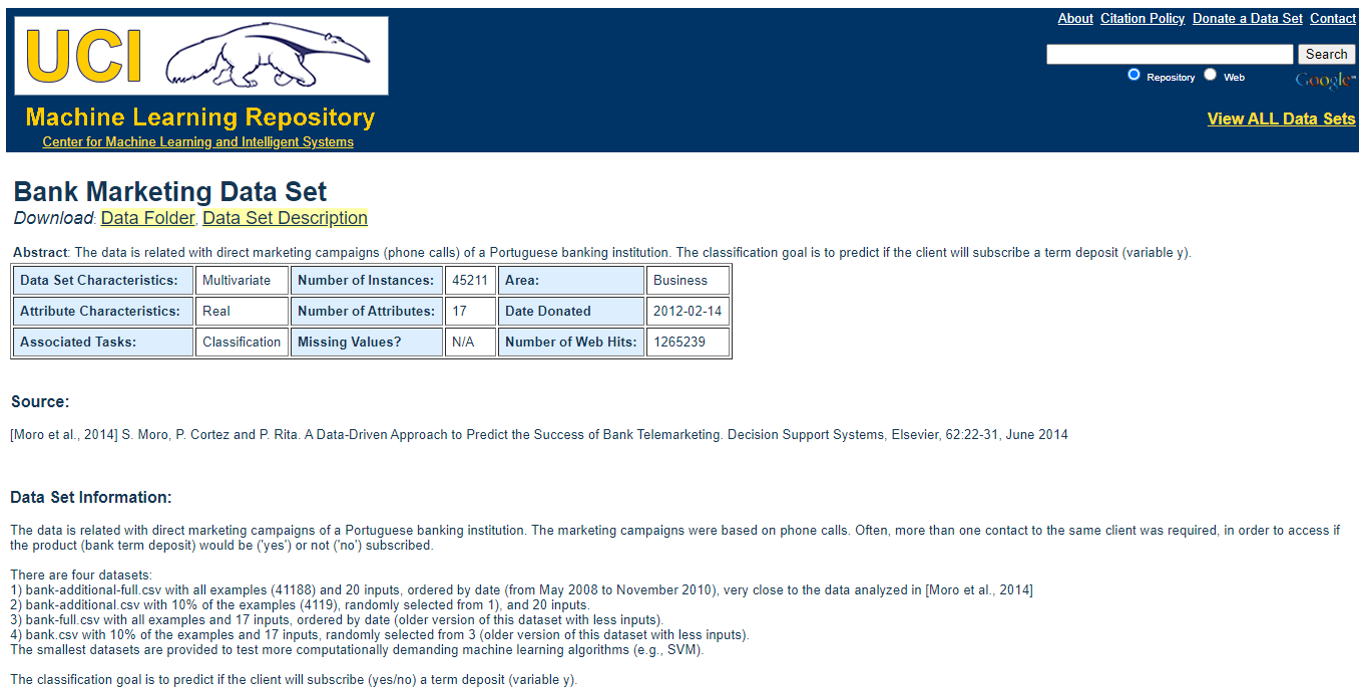
\includegraphics[scale = 0.65]{image/uci.png}
    		\caption{Bank Marketing Dataset được tổng hợp ở trang UCI}
    	\end{center}
    \end{figure}
    
    \begin{figure}[htp]
    	\begin{center}
    		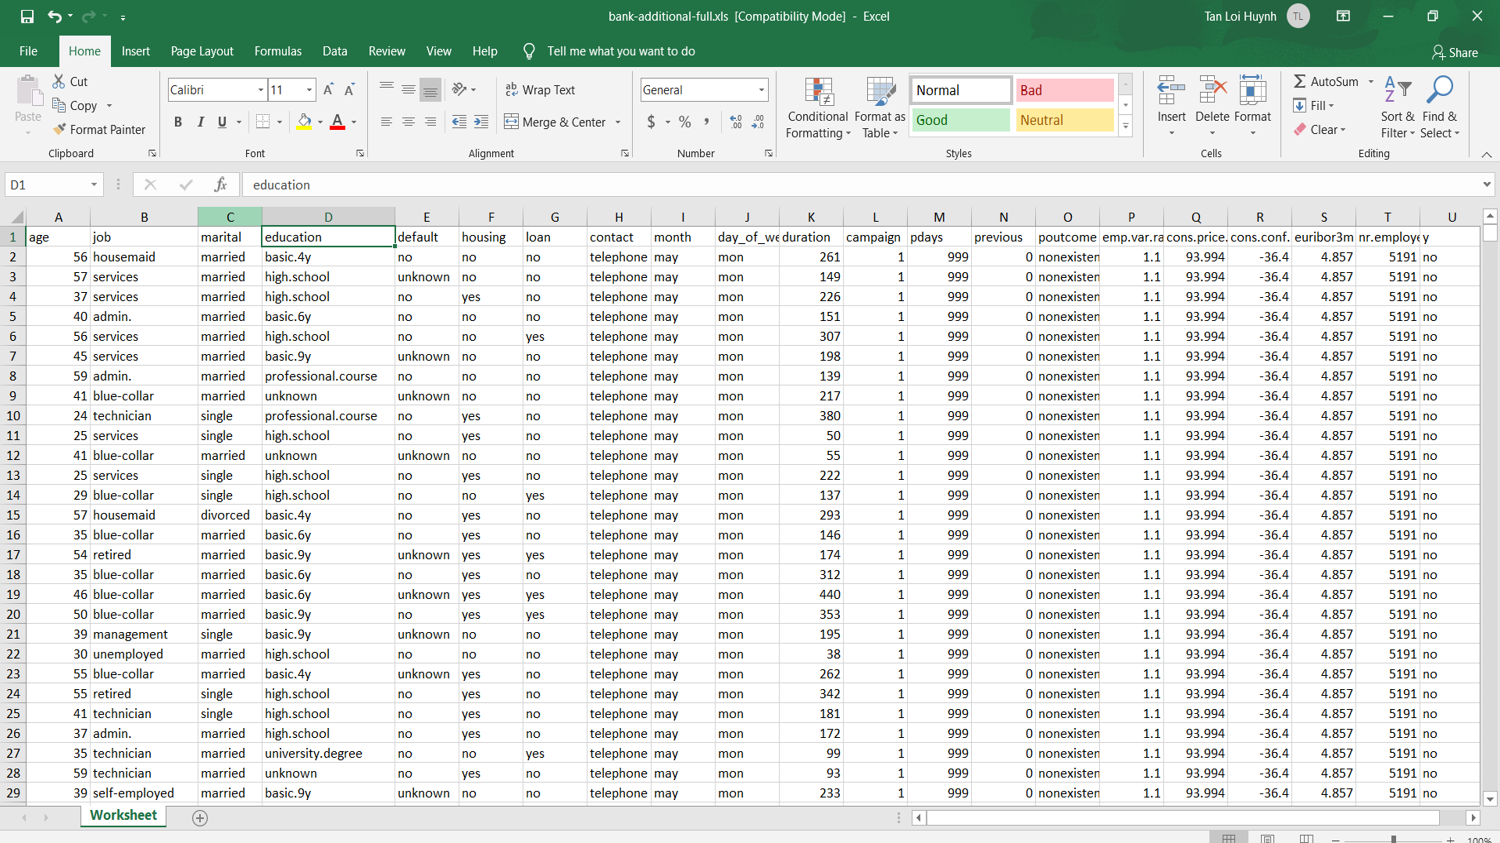
\includegraphics[scale = 0.65]{image/dataset.png}
    		\caption{Dữ liệu trong tập dataset có tên là \textit{bank-full.csv}}
    	\end{center}
    \end{figure}
    
%-------------------------------------------------------------------------------------------------------------
\pagebreak
%-------------------------------------------------------------------------------------------------------------

\fontsize{16}{10}\selectfont
\section{Đặc tả dữ liệu trong dataset}
    \fontsize{13}{10}\selectfont
    \begin{enumerate}
        \item age (Kiểu số - numeric)
        \item job: loại công việc (phân loại:"admin.","blue-collar", "entrepreneur", "housemaid", "management", "retired", "self-employed", "services", "student", "technician", "unemployed", "unknown").
        \item marital: tình trạng hôn nhân của khách hàng (phân loại: "divorced", "married", "single", "unknown").
        \item education (phân loại: "basic.4y", "basic.6y", "basic.9y", "high.school", "illiterate", "professional.course", "university.degree", "unknown").
        \item default: có tín dụng trong tình trạng vỡ nợ? (phân loại: "yes",  "no" và "unknown").
        \item housing: có cho vay mua nhà không? (phân loại: "yes",  "no" và "unknown").
        \item loan: có vay cá nhân không? (phân loại: "yes",  "no" và "unknown").
        \item contact: kiểu liên lạc (phân loại: "cellular", "telephone").
        \item month: tháng liên hệ cuối cùng trong năm (phân loại: “jan”, “feb”, “mar”,.., “nov”, “dec”).
        \item day\_of\_week: ngày liên hệ cuối cùng trong tuần (phân loại: “mon”, “tue”, “wed”, “thu”, “fri”).
        \item duration: thời lượng liên hệ cuối cùng, tính bằng giây (số). Lưu ý quan trọng: thuộc tính này ảnh hưởng nhiều đến mục tiêu đầu ra (ví dụ: nếu thời lượng = 0 thì y = ’không’). Khoảng thời gian không được biết trước khi cuộc gọi được thực hiện, cũng như sau khi kết thúc cuộc gọi, y hiển nhiên được biết. Do đó, đầu vào này chỉ nên được đưa vào cho các mục đích chuẩn và nên bị loại bỏ nếu mục đích là có một mô hình dự đoán thực tế.
        \item campaign: số liên hệ được thực hiện trong chiến dịch này và cho khách hàng này (kiểu số - numeric, bao gồm liên hệ cuối cùng)
        \item pdays: số ngày trôi qua sau khi khách hàng được liên hệ lần cuối từ một chiến dịch trước đó (kiểu dữ liệu số - numeric; 999 nghĩa là khách hàng không không có sự tương tác trước đó)
        \item previous: số lượng địa chỉ liên hệ của khách hàng được thực hiện trước khi thực hiện việc thu thập dữ liệu (kiểu dữ liệu số - numeric)
        \item poutcome: : kết quả của chiến dịch tiếp thị trước đó (phân loại:“failure”, “nonexistent”, “success”")
        \item emp.var.rate: tỷ lệ biến động việc làm - chỉ số hàng quý (kiểu dữ liệu số - numeric)
        \item cons.price.idx: chỉ số giá tiêu dùng - chỉ số hàng tháng (kiểu dữ liệu số - numeric)     
        \item cons.conf.idx:  chỉ số niềm tin của người tiêu dùng - chỉ số hàng tháng (kiểu dữ liệu - numeric)     
        \item euribor3m: euribor lãi suất 3 tháng - (kiểu dữ liệu số - numeric)
        \item nr.employed: số lượng nhân viên - chỉ số hàng quý (kiểu dữ liệu số - numeric)
        \item y - khách hàng đã đăng ký tiền gửi có kỳ hạn chưa? (nhị phân:"0" và "1")
    \end{enumerate}

\fontsize{16}{10}\selectfont
\section{Trưc quan bằng đồ thị và đánh giá tập dữ Bank Marketing}
\subsection{Trực quan hóa bằng đồ thị và đánh giá tập dữ liệu dựa trên số lượng khách hàng đăng ký một khoản tiền gửi có kỳ hạn}
    \fontsize{13}{10}\selectfont \textbf{$\star$\textit{ Trực quan hóa bằng đồ thị}}
        \begin{figure}[htp]
            \centering
            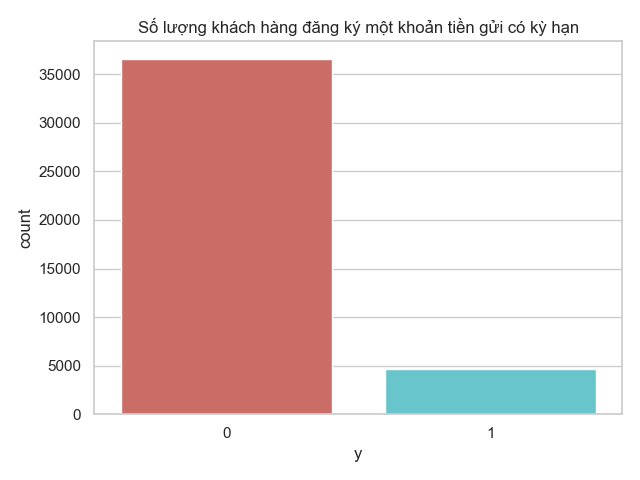
\includegraphics[scale = 0.7]{image/count_plot.png}
            \caption{Đồ thị biểu diễn số lượng khách hàng đăng ký một khoản tiền gửi có kỳ hạn từ dữ liệu trong dataset}
        \end{figure}
        
        \begin{figure}[htp]
            \centering
            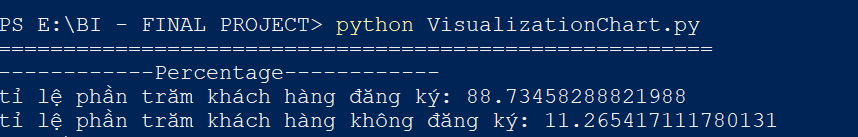
\includegraphics[scale = 0.75]{image/VC.png}
            \caption{Tỷ lệ khách hàng đăng ký và không đăng ký có trong dataset}
        \end{figure}
        
    %-------------------------------------------------------------------------------------------------------------
    \pagebreak
    %-------------------------------------------------------------------------------------------------------------

    \fontsize{13}{10}\selectfont \textbf{$\star$\textit{ Đánh giá}}
        \begin{enumerate}
            \item [- ] Số lượng khách hàng không đăng ký một khoản tiền gửi có kỳ hạn chiếm đa số trong tập dữ liệu.
            \item [- ] Biến phân loại dữ liệu bị nghiêng về một phía với tỷ lệ 90:10.
            \item [- ] Gây mất cân bằng dữ liệu (imbalanced dataset): 
            \begin{itemize}
                \item Mất cân bằng dữ liệu là một trong những hiện tượng phổ biến của bài toán phân loại nhị phân (binary classification) như dự đoán đăng ký, spam email, phát hiện gian lận, dự báo vỡ nợ, chuẩn đoán bệnh lý,… Trong trường hợp tỷ lệ dữ liệu giữa 2 classes là 50:50 thì được coi là cân bằng. Khi có sự khác biệt trong phân phối giữa 2 classes, chẳng hạn 60:40 thì dữ liệu có hiện tượng mất cân bằng.
                \item Trong tập dữ liệu trên, việc mất cân bằng dữ liệu nghiêm trọng xảy ra, tỷ lệ đưa ra ở đây là 90:10 sẽ dẫn tới ngộ nhận chất lượng mô hình. Khi đó thước đo đánh giá mô hình là độ chính xác (accuracy) có thể đạt được rất cao mà không cần tới mô hình. Như trường hợp trên, khách hàng đăng ký một khoản tiền gửi có kỳ hạn tất cả đều là nhóm đa số thì độ chính xác đã đạt được là 0.9. Do đó không nên lựa chọn độ chính xác làm chỉ số đánh giá mô hình để tránh lạc quan sai lầm về chất lượng.
                \item Với vấn đề này dẫn tới dự báo kém chính xác trên nhóm thiểu số. Bởi đa phần kết quả dự báo ra thường thiên về 1 nhóm là nhóm đa số và rất kém trên nhóm thiểu số. Trong khi tầm quan trọng của việc dự báo được chính xác một mẫu thuộc nhóm thiểu số lớn hơn nhiều so với dự báo mẫu thuộc nhóm đa số. Vì vậy cần một giải pháp để cải thiện độ chính xác cho mô hình trên nhóm thiểu số.
            \end{itemize}
        \end{enumerate}
                 
        %-------------------------------------------------------------------------------------------------------------
        \pagebreak
        %-------------------------------------------------------------------------------------------------------------

        \subsection{Trực quan hóa bằng đồ thị và đánh giá tập dữ liệu dựa trên số lượng khách hàng theo nghề nghiệp}
            \fontsize{13}{10}\selectfont \textbf{$\star$\textit{ Trực quan hóa bằng đồ thị}}
                \begin{figure}[htp]
                    \centering
                    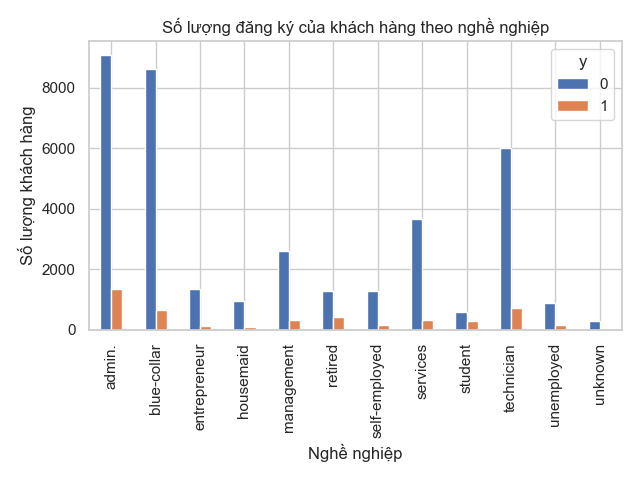
\includegraphics[scale = 0.8]{image/frequency_job.png}
                    \caption{Đồ thị thống kê số lượng khách hàng theo nghề nghiệp}
                \end{figure}
            
            \fontsize{13}{10}\selectfont \textbf{$\star$\textit{ Đánh giá}}
                \begin{enumerate}
                    \item [- ] Tần suất số lượng đăng ký của khách hàng thông qua các nghề nghiệp khác nhau biến động không đồng đều.
                    \item [- ] Admin: đạt tần suất cao nhất với cả hay trường hợp khách hàng đăng ký hay không đăng ký.
                    \item [- ] Unknown: đạt tần suất thấp nhất trường hợp khách hàng không đăng ký, tần suất gần như bằng 0 đối với khách hàng đăng ký.
                    \item [- ] Đây là một biến độc lập (independent variable) job mang nhiều yếu tố dự đoán cho biến phân loại y (outcome variable).
                \end{enumerate}
                 
        %-------------------------------------------------------------------------------------------------------------
        \pagebreak
        %-------------------------------------------------------------------------------------------------------------
    
        \subsection{Trực quan hóa bằng đồ thị và đánh giá tập dữ liệu dựa trên tỉ lệ khách hàng theo tình trạng hôn nhân}
            \fontsize{13}{10}\selectfont \textbf{$\star$\textit{ Trực quan hóa bằng đồ thị}}
                \begin{figure}[htp]
                    \centering
                    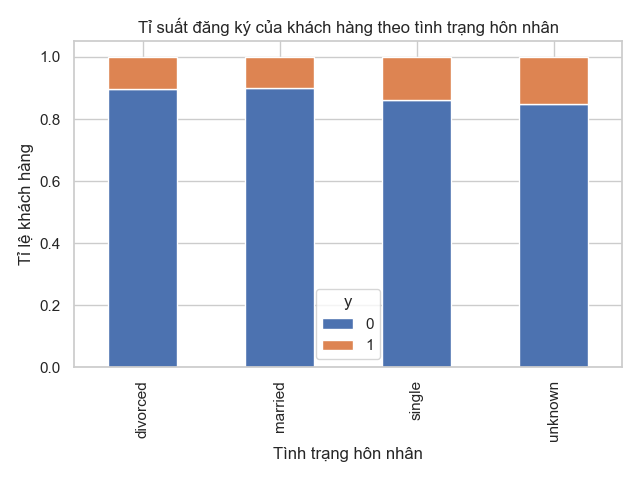
\includegraphics[scale = 0.8]{image/frequency_mariral.png}
                    \caption{Đồ thị thống kê tỉ lệ khách hàng đăng ký theo tình trạng hôn nhân}
                \end{figure}
            
            \fontsize{13}{10}\selectfont \textbf{$\star$\textit{ Đánh giá}}
                \begin{enumerate}
                    \item [- ] Single vs unknown: tỉ suất của hai tình trạng trên gần như bằng nhau đối với cả hai trường hợp khách hàng đăng ký hay không đăng ký.
                    \item [- ] Divorced vs married: tương tự hai tình trạng trên gần như bằng nhau đối với cả hai trường hợp.
                    \item [- ] Tỉ suất của các tình trạng hôn nhân không chênh lệch nhiều so với các trường hợp khác.
                    \item [$\Rightarrow$] \textbf{\underline{\textit{Kết luận}}}: biến độc lập (independent variable) marital không phải là một yếu tố dự đoán cho biến phân loại y (outcome variable).
                \end{enumerate}
                 
        %-------------------------------------------------------------------------------------------------------------
        \pagebreak
        %-------------------------------------------------------------------------------------------------------------

        \subsection{Trực quan hóa bằng đồ thị và đánh giá tập dữ liệu dựa trên tỉ lệ khách hàng theo trình độ giáo dục}
            \fontsize{13}{10}\selectfont \textbf{$\star$\textit{ Trực quan hóa bằng đồ thị}}
                \begin{figure}[htp]
                    \centering
                    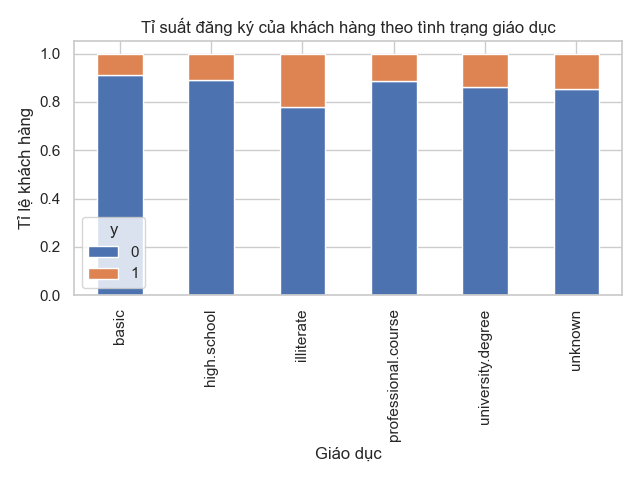
\includegraphics[scale = 0.8]{image/frequency_education.png}
                    \caption{Đồ thị thống kê tỉ lệ khách hàng đăng ký theo trình độ giáo dục}
                \end{figure}
            
            \fontsize{13}{10}\selectfont \textbf{$\star$\textit{ Đánh giá}}
                \begin{enumerate}
                    \item [- ] Illiterate: đạt tỉ suất thấp nhất đối với trường hợp khách hàng không đăng ký, đạt tỉ suất cao nhất đối với trường hợp khách hàng đăng ký.
                    \item [- ] Basic (nhóm dữ liệu từ basic.4y, basic.6y và basic.9y): đạt tỉ suất cao nhất đối với trường hợp khách hàng không đăng ký, đạt tỉ suất thấp nhất đối với trường hợp khách hàng đăng ký.
                    \item [$\Rightarrow$] \textbf{\underline{\textit{Kết luận}}}: biến độc lập (independent variable) education là một yếu tố dự đoán tốt cho biến phân loại y (outcome variable).
                \end{enumerate}
                 
        %-------------------------------------------------------------------------------------------------------------
        \pagebreak
        %-------------------------------------------------------------------------------------------------------------

        \subsection{Trực quan hóa bằng đồ thị và đánh giá tập dữ liệu dựa trên số lượng khách hàng đăng ký theo ngày}
            \fontsize{13}{10}\selectfont \textbf{$\star$\textit{ Trực quan hóa bằng đồ thị}}
                \begin{figure}[htp]
                    \centering
                    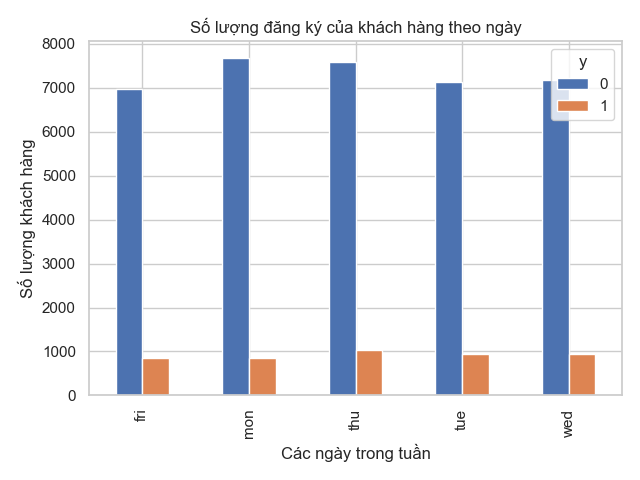
\includegraphics[scale = 0.8]{image/frequency_dayofweek.png}
                    \caption{Đồ thị thống kê  số lượng khách hàng đăng ký theo ngày}
                \end{figure}
            
            \fontsize{13}{10}\selectfont \textbf{$\star$\textit{ Đánh giá}}
                \begin{enumerate}
                    \item [- ] Tần suất khách hàng đăng ký theo các ngày trong tuần gần chênh lệch rất ít so với các ngày còn lại.
                    \item [- ] Do tập dữ liệu đang bị mất cân bằng nghiêm trọng nghiên về y = 0, việc tần suất khách hàng không đăng ký chênh lệch sẽ không tạo ra ảnh hưởng so với trường hợp khách hàng đăng ký nên sẽ bỏ qua.
                    \item [$\Rightarrow$] \textbf{\underline{\textit{Kết luận}}}: tương tự như marital, biến độc lập (independent variable) dayofweek không phải là yếu tố dự toán tốt cho biến phân loại y (outcome variable).
                \end{enumerate}
            
        %-------------------------------------------------------------------------------------------------------------
        \pagebreak
        %-------------------------------------------------------------------------------------------------------------
        
        \subsection{Trực quan hóa bằng đồ thị và đánh giá tập dữ liệu dựa trên số lượng khách hàng đăng ký theo tháng}
            \fontsize{13}{10}\selectfont \textbf{$\star$\textit{ Trực quan hóa bằng đồ thị}}
                \begin{figure}[htp]
                    \centering
                    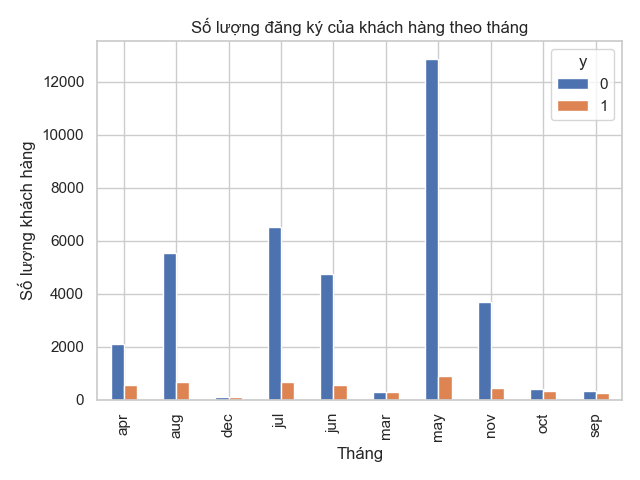
\includegraphics[scale = 0.8]{image/frequency_month.png}
                    \caption{Đồ thị thống kê  số lượng khách hàng đăng ký theo tháng}
                \end{figure}
            
            \fontsize{13}{10}\selectfont \textbf{$\star$\textit{ Đánh giá}}
                \begin{enumerate}
                    \item [- ] May: đạt tần suất cao nhất trong cả 2 trường hợp khách hàng đăng ký và không đăng ký.
                    \item [- ] Dec: đạt tần suất thấp nhất trong cả 2 trường hợp khách hàng đăng ký và không đăng ký.
                    \item [- ] Tần suất của các tháng trong năm thay đổi luân phiên không đồng đều.
                    \item [$\Rightarrow$] \textbf{\underline{\textit{Kết luận}}}: biến độc lập (independent variable) month là một yếu tố dự đoán tốt cho biến phân loại y (outcome variable).
                \end{enumerate}
            
        %-------------------------------------------------------------------------------------------------------------
        \pagebreak
        %-------------------------------------------------------------------------------------------------------------
        
        \subsection{Trực quan hóa bằng đồ thị và đánh giá tập dữ liệu dựa trên số lượng khách hàng đăng ký theo tình trạng tiếp thị trước đó}
            \fontsize{13}{10}\selectfont \textbf{$\star$\textit{ Trực quan hóa bằng đồ thị}}
                \begin{figure}[htp]
                    \centering
                    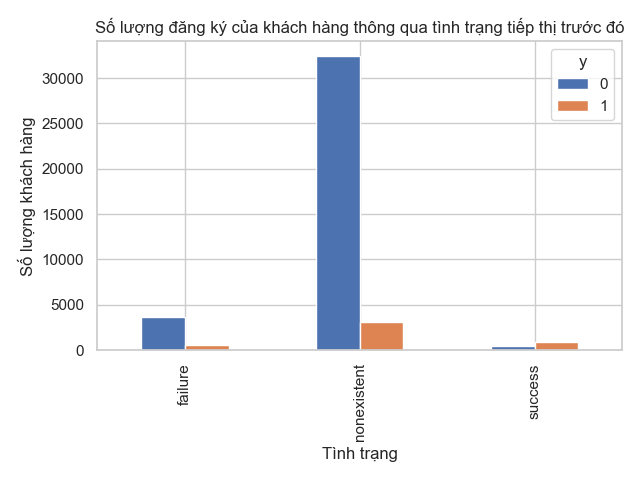
\includegraphics[scale = 0.8]{image/frequency_poutcome.png}
                    \caption{Đồ thị thống kê  số lượng khách hàng đăng ký theo tình trạng tiếp thị trước đó}
                \end{figure}
            
            \fontsize{13}{10}\selectfont \textbf{$\star$\textit{ Đánh giá}}
                \begin{enumerate}
                    \item [- ] Nonexistent: đạt tần suất cao nhất trong cả 2 trường hợp khách hàng đăng ký và không đăng ký.
                    \item [- ] Success: đạt tần suất thấp nhất trong cả 2 trường hợp khách hàng đăng ký và không đăng ký.
                    \item [$\Rightarrow$] \textbf{\underline{\textit{Kết luận}}}: tương tự như các biến độc lập khác (independent variable), poutcome là yếu tố dự đoán tốt cho biến phân loại y (outcome variable).
                \end{enumerate}
            
        %-------------------------------------------------------------------------------------------------------------
        \pagebreak
        %-------------------------------------------------------------------------------------------------------------
        
        \subsection{Trực quan hóa bằng đồ thị và đánh giá tập dữ liệu dựa trên số lượng khách hàng đăng ký theo độ tuổi}
            \fontsize{13}{10}\selectfont \textbf{$\star$\textit{ Trực quan hóa bằng đồ thị}}
                \begin{figure}[htp]
                    \centering
                    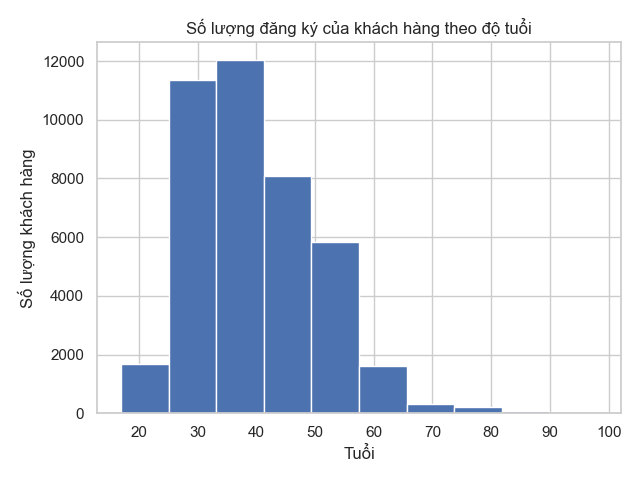
\includegraphics[scale = 0.8]{image/hist_age.png}
                    \caption{Đồ thị thống kê  số lượng khách hàng đăng ký theo độ tuổi}
                \end{figure}
            
            \fontsize{13}{10}\selectfont \textbf{$\star$\textit{ Đánh giá}}
                \begin{enumerate}
                    \item [- ] Hầu hết các khách hàng ở độ tuổi từ 30 đến 50.
                    \item [- ] Sự ảnh hưởng của độ tuổi khách hàng đối với chiến dịch tiếp thị mang tầm ảnh hưởng cao.
                    \item [$\Rightarrow$] \textbf{\underline{\textit{Kết luận}}}: biến độc lập (independent variable) age cũng có thể là một yếu tố dự đoán tốt cho biến phân loại y (outcome variable).
                \end{enumerate}
            
            \fontsize{13}{10}\selectfont\textbf{$\Longrightarrow$ \underline{\underline{{TỔNG KẾT}}}}:
                \begin{enumerate}
                    \item [- ] Trong tập dữ liệu, các biến độc lập khác nhau mang yếu tố dự toán tốt cho biến phân loại. Cần một giải pháp tối ưu để mang lại sự dự đoán biến phân loại y đạt độ chính xác (accuracy) cao nhất.
                    \item [- ] Tập dữ liệu bị mất cân bằng (imbalanced dataset), cần đề ra giải pháp để tối ưu được số lượng cũng như cân bằng dữ liệu 2 bên classes.
                \end{enumerate}
                
    %-------------------------------------------------------------------------------------------------------------
    \pagebreak
    %-------------------------------------------------------------------------------------------------------------

    \fontsize{16}{10}\selectfont
    \section{Xử lý dataset}
        \subsection{Quá trình xử lý thuật toán}
        \fontsize{13}{10}\selectfont\paragraph{}
            Quá trình xử lý dataset trải qua tuần tự các bước sau:
            \begin{enumerate}
                    \item [- ] Đơn giản hóa dữ liệu: Ở biến độc lập \textit{education}, thực hiện việc gôm nhóm các dữ liệu \textit{basic.4y}, \textit{basic.6y} và \textit{basic.9y} thành \textit{basic}.
                    
                    \begin{figure}[htp]
                        \centering
                        \tab[1cm]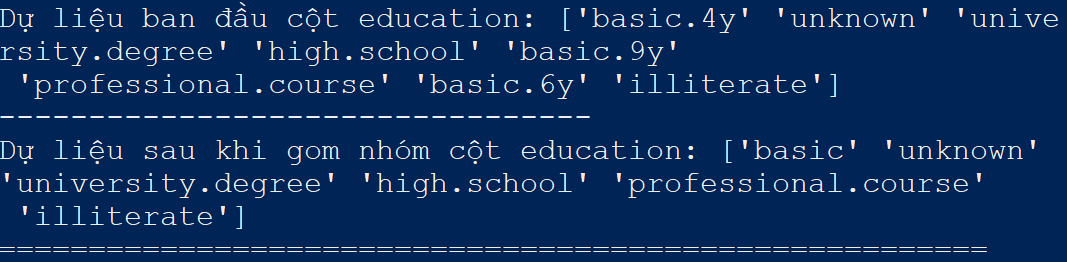
\includegraphics[scale = 0.72]{image/VC_1.png}
                        \caption{Dữ liệu trước và sau khi đơn giản hóa ở cột education}
                    \end{figure}
                    
                    \item [- ]	Tạo biến giả (Dummy variable):
                        \begin{itemize}
                            \item Biến giả là biến độc lập được đưa vào mô hình hồi qui để giải thích các yếu tố định tính.
                            \item Chuyển đổi biến độc lập loại chuỗi thành các biến độc lập loại số dạng nhị phân (1 hoặc 0).
                            \item [$\diamond$] Ví dụ: Từ biến độc lập marital ta khởi tạo thành một biến giả dạng nhị phân 
                            \newline\tab[1.25cm] marital = married
                            \newline\tab[1.25cm] marital-married = 1 nếu khách hàng đó có kết hôn
                            \newline\tab[1.25cm] marital-married = 0 nếu khách hàng không có kết hôn
                        \end{itemize}
                        
                    \item [- ] Các biến độc lập cần xử lý dữ liệu:
                        \begin{itemize}
                            \item Job:
                                \newline\tab “admin”, “blue-collar”, “entrepreneur”, “housemaid”,
                                \newline\tab “management”, “retired”, “self-employed”, “services”,
                                \newline\tab “student”, “technician”, “unemployed”, “unknown”
                            \item marital:
                                \newline\tab “divorced”, “married”, “single”, “unknown”
                            \item education:
                                \newline\tab “basic”, “high.school”, “illiterate”, “professional.course”, 
                                \newline\tab “university.degree”, “unknown”
                            \item default:
                                \newline\tab “no”, “yes”, “unknown”
                                
                            \item housing:
                                \newline\tab “no”, “yes”, “unknown”
                            \item loan:
                                \newline\tab “no”, “yes”, “unknown”
                            \item contact:
                                \newline\tab “cellular”, “telephone”
                            \item month:
                                \newline\tab “jan”, “feb”, “mar”,..., “nov”, “dec”
                            \item day\_of\_week:
                                \newline\tab “mon”, “tue”, “wed”, “thu”, “fri”
                            \item poutcome:
                                \newline\tab “failure”, “nonexistent”, “success”
                        \end{itemize}
                        
                    \begin{figure}[htp]
                        \centering
                        \tab[1.25cm]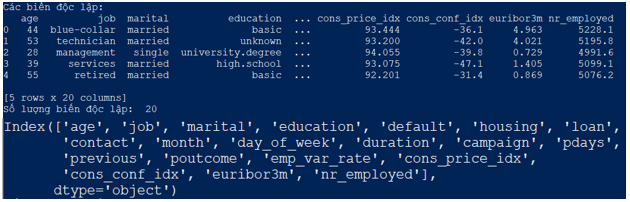
\includegraphics[scale = 0.96]{image/VC_2.png}
                        \caption{Dữ liệu ban đầu trước khi tạo các biến giả}
                    \end{figure}
                    
                    \begin{figure}[htp]
                        \centering
                        \tab[1.25cm]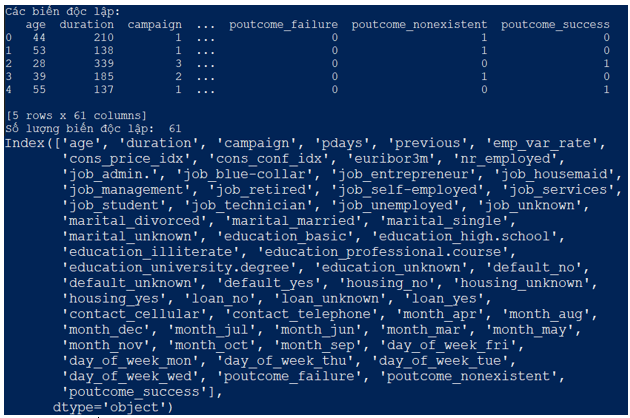
\includegraphics[scale = 0.96]{image/VC_3.png}
                        \caption{Dữ liệu sau khi xử lý và khởi tạo các biến giả}
                    \end{figure}
                \end{enumerate}
            
    %-------------------------------------------------------------------------------------------------------------
    \pagebreak
    %-------------------------------------------------------------------------------------------------------------

        \subsection{Các giải pháp sử dụng trong quá trình xử lý dataset}   
            \begin{enumerate}
                \item [- ] Giải pháp Oversampling và phương pháp SMOTE:
                    \begin{itemize}
                        \item Tạo dữ liệu mẫu giả cho tập thiểu số sao cho số phần tử của nó được nhiều lên bằng cách là lặp lại mỗi điểm trong nhóm thiểu số nhiều lần.
                        \item SMOTE (Synthetic Minority Over-sampling): là phương pháp sinh mẫu nhằm gia tăng kích thước mẫu của nhóm thiểu số trong trường hợp xảy ra mất cân bằng mẫu. Để gia tăng kích thước mẫu, với mỗi một mẫu thuộc nhóm thiểu số sẽ lựa chọn ra k mẫu láng giềng gần nhất với nó và sau đó thực hiện tổ hợp tuyến tính để tạo ra mẫu giả lập. Phương pháp để lựa chọn ra các láng giềng của một quan sát có thể dựa trên thuật toán KNN hoặc SVM.
                        \begin{figure}[htp]
                            \centering
                            \tab[1.25cm]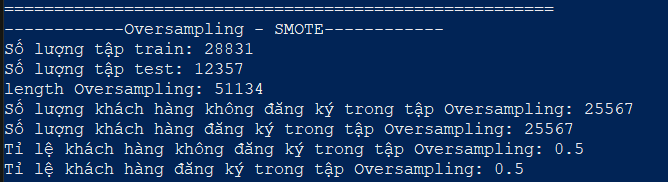
\includegraphics[scale = 1.1]{image/VC_4.png}
                            \caption{Kết quả sau khi áp dung phương pháp SMOTE}
                        \end{figure}
                    \end{itemize}
            
        %-------------------------------------------------------------------------------------------------------------
        \pagebreak
        %-------------------------------------------------------------------------------------------------------------
                        
            \item [- ] Giải pháp RFE (Recursive Feature Elimination): Đánh giá được mức độ tác động (quan trọng) của các thuộc tính để từ đó chọn ra được tập thuộc tính tốt nhất để xây dựng mô hình, giúp làm tăng hiệu suất và rút ngắn thời gian huấn luyện mô hình.
                \begin{itemize}
                    \item Áp dụng phương pháp RFE để đánh giá 61 thuộc tính (61 biến độc lập):
                        \begin{figure}[htp]
                            \centering
                            \tab[1.25cm]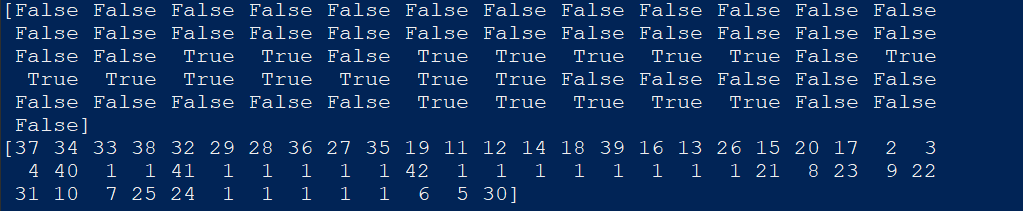
\includegraphics[scale = 0.75]{image/VC_5.png}
                            \caption{Kết quả sau khi áp dung phương pháp RFE}
                        \end{figure}
                    \item Chọn vị trí các thuộc tính có rank = 1:
                        \begin{figure}[htp]
                            \centering
                            \tab[1.25cm]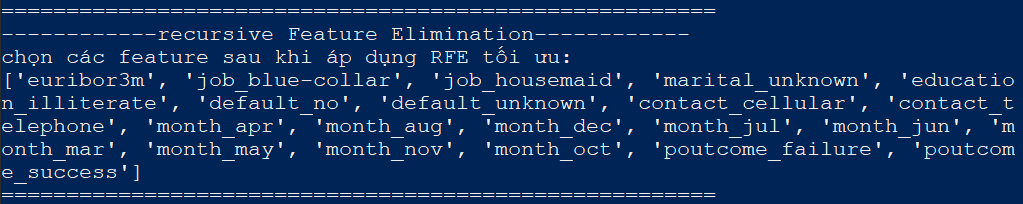
\includegraphics[scale = 0.75]{image/VC_6.png}
                        \end{figure}
                \end{itemize}
        \end{enumerate}
        
%-------------------------------------------------------------------------------------------------------------
\pagebreak
%-------------------------------------------------------------------------------------------------------------

%-------------------------------------------------------------------------------------------------------------
%---------------Chapter 3 -----------------------
\fontsize{18}{10}\selectfont
\chapter{THUẬT TOÁN HỒI QUY LOGISTIC}
    \fontsize{16}{10}\selectfont
    \section{Sự xuất hiện của hồi quy logistic}

        \begin{wrapfigure}{l}[-0.65cm]{0.25\linewidth}
            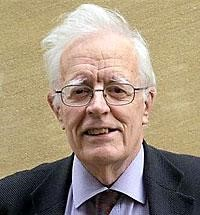
\includegraphics[scale=0.75]{image/s_d_roxbee.jpg}
            \caption{\centering Sir David Roxbee Cox}
        \end{wrapfigure}
        
        \fontsize{13}{10}\selectfont\paragraph{}
             Sir David Roxbee Cox (sinh ngày 15 tháng 7 năm 1924) là một nhà thống kê người Anh nổi tiếng. Ông đã có những đóng góp tiên phong và quan trọng trong nhiều lĩnh vực thống kê và xác suất ứng dụng và một trong những thuật toán nổi tiếng nhất và được xử dụng rộng rãi và phổ biến nhất trong việc lĩnh vực y học cũng như các lĩnh vực thống kê và phân tích dữ liệu để đưa ra quyết định với xác suất rủi ro thấp nhất. Và thuật toán hữu dụng ấy đã tạo nên nhiều bước tiếng trong lĩnh vực thống kê, cải thiện và hỗ trợ rất nhiều cho ngành phân tích dữ liệu, tính toán thông minh.
        
        \fontsize{13}{10}\selectfont\paragraph{}
            Trong thống kê , mô hình logistic (hoặc mô hình logit) được sử dụng để mô hình hóa xác suất của một lớp hoặc sự kiện nhất định tồn tại như đạt/không đạt, thắng/thua, sống/chết hoặc khỏe mạnh/bệnh tật (tùy thuộc vào thuộc tính của tập dữ liệu đang xét). Điều này có thể được mở rộng để mô hình hóa một số lớp sự kiệ. Mỗi đối tượng được phát hiện sẽ được gán một xác suất từ 0 đến 1, với tổng là một.
            
    %-------------------------------------------------------------------------------------------------------------
    \pagebreak
    %-------------------------------------------------------------------------------------------------------------
    
    \section{Ý nghĩa và lợi ích}
        \fontsize{13}{10}\selectfont\paragraph{}
            Hồi quy từ lâu đã trở thành một phần không thể thiếu trong Data analysis liên quan đến việc tìm hiểu và phân tích mối quan hệ giữa các đối tượng nghiên cứu thể hiện qua biến mục tiêu (biến y) và các biến độc lập (biến giải thích - các biến x).
        \fontsize{13}{10}\selectfont\paragraph{}
            Lợi thế mô hình hồi quy logistic đó chính là có thể áp dụng cho nhiều mô hình nghiên cứu, nhiều software có thể dùng để ước tính tham số.
    
    \section{Ứng dụng của hồi quy logistics}
        \fontsize{13}{10}\selectfont\paragraph{}
            Hồi quy logistic dự báo khả năng xảy ra của một sự kiện, tình huống trong tương lai. Nó được ứng dụng trong nhiều lĩnh vực khác nhau không chỉ riêng trong thống kê, có thể nói đến như: lĩnh vực khai phá dữ liệu – Data mingning, lĩnh vực học máy – Machine Learning, trong lĩnh vực ngân hàng dùng để đánh giá rủi ro tín dụng,...
        
        \fontsize{13}{10}\selectfont\paragraph{}
            Việc xuất hiện của hồi quy logistic đã giúp giải quyết rất nhiều vấn đề cuộc sống.Đặc biệt là trong các nghiên cứu quan trọng việc áp dụng hồi quy logistic đã giúp hạn chế bớt sai xót, rủi ro và nâng cao độ chính xác. Các nghiên cứu có áp dụng logistics regression có thể kể đến như là: Nghiên cứu mối tương quan giữa phơi nhiễm chất độc da cam và ung thư tuyến tiền liệt.
        
        \fontsize{13}{10}\selectfont\paragraph{}
            Cụ thể, vào năm 2004, Giri và đồng nghiệp đã tiến hành một nghiên cứu sơ bộ để thẩm định mối liên hệ giữa phơi nhiễm chất độc màu da cam (Agent Orange – AO) và nguy cơ ung thư tuyến tiền liệt (prostate cancer risk) ở các cựu chiến binh Mĩ từng tham chiến ở Việt Nam trước đây.
        
        \fontsize{13}{10}\selectfont\paragraph{}
            Hồi quy logistic là phương pháp hồi quy thông dụng nhất, áp dụng cho các biến mục tiêu không phải là biến định lượng liên tục, trong đó:
            \vspace{0.2cm}\newline\tab[1.5cm]• Biến outcome là biến phân loại, nói cách khác là biến nhị phân
            \vspace{0.2cm}\newline\tab[1.5cm]• Biến độc lập hay biến tiên lượng có thể là biến liên tục hay biến nhị phân.
            \vspace{0.2cm}\newline\tab[0.25cm]Biến (hay dữ liệu) thường sẽ có hai dạng chính đó là: dạng định tính (qualitative/categorical variable) và dạng định lượng (quantitative/numerial variable). Ngoài ra, còn có biến nhị phân (binary variable).
            \vspace{0.2cm}\newline\tab[1.5cm]• Biến định tính (biến phân loại): là biến phản ánh tính chất hoặc loại hình, không có biểu hiện trực tiếp bằng con số (\textit{ví dụ}: tình trạng hôn nhân, giới tính, nghề nghiệp)
            \vspace{0.2cm}\newline\tab[1.5cm]• Biến định tính được phân làm 2 dạng: 
            \vspace{0.2cm}\newline\tab[2.5cm]◦ Định danh (Nominal): nghề nghiệp – bác sĩ, giáo viên,..
            \vspace{0.2cm}\newline\tab[2.5cm]◦ Thứ bậc (Ordinal): thứ hạng - hạng nhất, hạng nhì,...
            \vspace{0.2cm}\newline\tab[1.5cm]• Biến độc lập hay biến tiên lượng có thể là biến liên tục hay biến nhị phân.Tuy trên lý thuyết thì biến tiên lượng không có sai số ngẫu nhiên nhưng thực tế thì những sai số đó có tồn tại. 
            \vspace{0.2cm}\newline\tab[1.5cm]• Biến định lượng là biến thể hiện trực tiếp bằng con số (\textit{ví dụ}: chiều cao, cân nặng, tuổi,..). Biến định lượng được phân làm 2 dạng: 
            \vspace{0.2cm}\newline\tab[2.5cm]◦ Rời rạc (Discrete): dân số,..
            \vspace{0.2cm}\newline\tab[2.5cm]◦ Liên tục (Continuous): nhiệt độ, cân nặng, chiều cao..
            \vspace{0.2cm}\newline\tab[1.5cm]• Biến nhị phân là biến chỉ có 2 giá trị, 2 biểu hiện không trùng nhau của một đơn vị. Nếu đơn vị không chứa giá trị này, thì phải chứa giá trị còn lại của biến (\textit{ví dụ}: Có/Không, Đúng/sai, Sống/chết, Dừng lại/ tiếp tục).
            \vspace{0.2cm}\newline\tab[1.5cm]• Biến nhị phân chia làm 2 loại: đối xứng (Symmetric) và bất đối xứng (Asymmetric)
            
        \begin{center}
            \begin{figure}[htp]
                \begin{center}
                    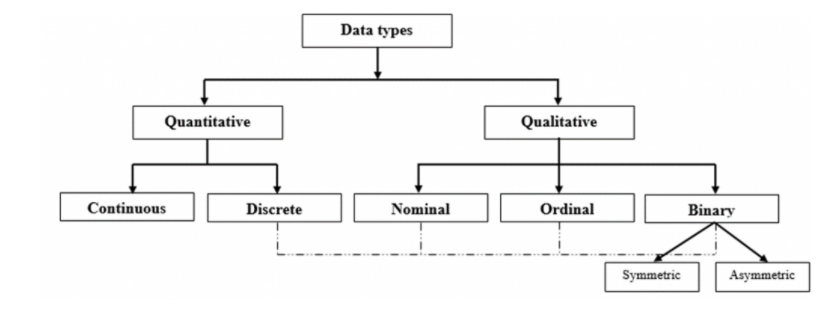
\includegraphics[scale = 0.75]{image/sodophanloaibien.png}
                \end{center}
                \caption{Sơ đồ phân loại các biến}
            \end{figure}
        \end{center}
        
    \section{Mô hình hồi quy logistic}
    \fontsize{13}{10}\selectfont
    \begin{enumerate}
        \item [- ] Probability (p); là xác suất của một biến cố trong một thời gian (p sẽ dao động trong khoảng từ 0 đến 1).
        \item [- ] odds: là tỷ số giữa xác suất biến cố xảy ra chia cho xác suất biến cố không xảy ra. Odds được xem là một biến liên tục, giá trị của odds không nhất thiết phải nằm tròn khoản từ 0 đến 1 và giá trị của odds bằng 1 khi và chỉ khi p = 0.5. Để tính odds chúng ta áp dụng công thức: $odd = \frac{p}{1 - p}$ 
                
        %-------------------------------------------------------------------------------------------------------------
        \pagebreak
        %-------------------------------------------------------------------------------------------------------------
        
        \item [- ] odds ratio: là tỷ số giữa 2 odd vầ được xác định bằng công thứ; $ \frac{odd_1}{odd_2} = \frac{P(X,Y)P(\overline{X},\overline{Y}}{P(X,\overline{Y}P(\overline{X},Y)}$

        \vspace{0.2cm}\tab\textit{\textbf{Ví dụ:} Xét trường hợp 5 người cùng đến xét nghiệm ung thư phổi và kết quả trả về là 1 người trong số họ mắc bệnh.}\vspace{0.2cm}
        \newline\tab\quad Ta có: $p = \frac{1}{5} = 0.2$\\
        \vspace{0.2cm}\newline\tab\quad$\Rightarrow odds = \frac{p}{1 - p} = \frac{0.2}{1-0.2} = 0.25$
        \item [- ] logit chính là $\log(odds)$ và được xác định bằng công thức: \\\tab\textbf{$logit(p) = \log(odds) = \log(\frac{p}{1 - p})$}
        \item [- ] Nếu gọi X là biến tiên lượng và p là xác suất của một biến cố (outcome) thì mô hình hồi quy logistic sẽ được phát biểu như sau:
        \vspace{0.2cm}\newline\tab[6cm] $logit(p) = \alpha + \beta X$ \newline\tab[5cm] hay: \vspace{0.2cm}\newline\tab[6cm] $\log(\frac{p}{1 - p}) = \alpha + \beta X$
        \item [- ] Phương trình tổng quát để ước lượng xác suất dạng đa biến như sau:
        \vspace{0.2cm}\newline\tab[2cm] $\hat{y} = $ Ước lượng P( y = 1 $\mid x_1, x_2,...,x_p) = \frac{e^{\alpha + \beta_1x_1 + \beta_2x_2 + ... + \beta_px_p}}{1 + e^{\alpha + \beta_1x_1 + \beta_2x_2 + ... + \beta_px_p}}$
        Trong đó:
        \begin{itemize}
            \item $\alpha$ là hệ số chặn (intercept). Giá trị của z khi tất cả các biến độc lập bằng 0 (X=0).
            \item $\beta$ là hệ số hồi qui (regression cofficients) của các  yếu tố nguy cơ (còn gọi là biến độc lập) x1, x2,…, xk. Hệ số hồi qui cho biết độ mạnh cũng như chiều của sự ảnh hưởng của các yếu tố nguy cơ đến xác suất xảy ra sự kiện nghiên cứu. Nếu hệ số hồ qui dương thì yếu tố nguy cơ làm tăng khả năng (xác suất) xảy ra của sự kiện nghiên cứu và ngược lại.
        \end{itemize}
        \begin{center}
            \begin{figure}[htp]
                \begin{center}
                    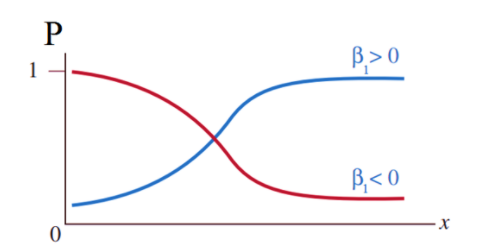
\includegraphics[scale = 0.9]{image/dothiphuongtrinhuocluongxacsuat.PNG}
                \end{center}
                \caption{Đồ thị phương trình ước lượng xác suất}
            \end{figure}
        \end{center}
    \end{enumerate}
             
    %-------------------------------------------------------------------------------------------------------------
    \pagebreak
    %-------------------------------------------------------------------------------------------------------------

    \fontsize{16}{10}\selectfont
    \section{Thực nghiệm trên một biến độc lập}
    \fontsize{13}{10}\selectfont\paragraph{}
        Chọn blue-collar ở cột job là biến X $\iff$ X $\to$ Y \vspace{0.2cm}\\
        \tab[0.25cm] Vấn đề đặt ra : Nghiên cứu sự tương quan giữa nghề nghiệp của khách hàng và việc đăng ký một khoảng tiền gửi có kỳ hạn cho ngân hàng.
        
        \begin{center}
            \begin{figure}[htp]
                \begin{center}
                    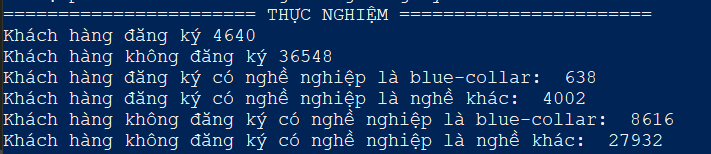
\includegraphics[scale = 0.9]{image/LR_1.png}
                \end{center}
                \caption{Dữ liệu thực nghiệm lấy từ dataset}
            \end{figure}
        \end{center}
        
        \begin{center}
            \begin{figure}[htp]
                \begin{center}
                    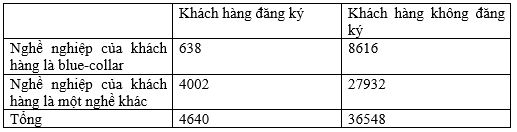
\includegraphics[scale = 1]{image/datathucnghiem.PNG}
                \end{center}
                \caption{Thống kê dữ liệu thực nghiệm lấy từ dataset}
                \fontsize{13}{15}\selectfont Ta có:
                    \vspace{0.2cm}\newline\tab[1cm] Odd khách hàng đăng ký có nghề nghiệp là blue-collar là ($odd_1$): $\frac{638}{8616} = 0.074$
                    \vspace{0.2cm}\newline\tab[1cm] Odd khách hàng đăng ký có nghề nghiệp là một nghề khác là ($odd_0$): $\frac{4002}{27932} = 0.143$
                    \vspace{0.2cm}\newline\tab[1cm] Odds ratio khách hàng đăng ký có nghề nghiệp là blue-collar so với khách hàng đăng ký có nghề nghiệp là một nghề khác là: $\frac{0.074}{0.143} = 0.517$\\
            \end{figure}
        \end{center}
        
        %-------------------------------------------------------------------------------------------------------------
        \pagebreak
        %-------------------------------------------------------------------------------------------------------------
    
        \fontsize{13}{10}\selectfont \textbf{$\star$\textit{ Đưa ra quyết định:}}
            \vspace{0.2cm}\newline Ta có phương trình tổng quát:
            \vspace{0.2cm}\newline\tab[1cm] $\hat{y} = $ Ước lượng P( y = 1 $\mid x_1, x_2,...,x_p) = \frac{e^{\alpha + \beta_1x_1 + \beta_2x_2 + ... + \beta_px_p}}{1 + e^{\alpha + \beta_1x_1 + \beta_2x_2 + ... + \beta_px_p}}$
            \vspace{0.2cm}\newline\tab[1cm] $\Rightarrow $ P = $\frac{e^{\alpha + \beta x}}{1 + e^{\alpha + \beta x}}$ với x là biến độc lập job\_blue-collar. Với x = 0 (nghề nghiệp là một nghề khác):
            \vspace{0.2cm}\newline\tab[2.5cm] $Odd_0 = e^{\alpha + \beta} = e^{\alpha} = 0.143 \Rightarrow \alpha = -0.845$
            \vspace{0.2cm}\newline\tab[2.5cm] $Odd_1 = e^{\alpha + \beta} = e^{\alpha + \beta} = 0.074 \Rightarrow \alpha + \beta = -1.131$
            \vspace{0.2cm}\newline\tab[2.5cm] $\Rightarrow $Odds ratio (OR) = $\frac{Odd_1}{Odd_0} = \frac{e^{\alpha + \beta}}{e^{\alpha}} = e^{\beta} = 0.517 \Rightarrow \beta = -0.287$
        \fontsize{13}{10}\selectfont \vspace{0.2cm}\newline\textbf{$\star$\textit{ Phương trình ước lượng xác suất:}}
            \vspace{0.2cm}\newline\tab[2.5cm] $\Rightarrow P = \frac{e^{\alpha + \beta x}}{1 + e^{\alpha + \beta x}} = \frac{e^{-0.845 - 0.287 * 1}}{1 + e^{-0.845 - 0.287 * 1}} = 0.244$\\
        \fontsize{13}{10}\selectfont\textbf{$\Longrightarrow$ \underline{{Kết luận}}}: Tương tự với các biến độc lập khác, ta lập được phương trình ước lượng xác xuất cho đa biến để giải quyết bài toán trên.
    
    %-------------------------------------------------------------------------------------------------------------
    \pagebreak
    %-------------------------------------------------------------------------------------------------------------
    
    \fontsize{16}{10}\selectfont
    \section{Demo}
    \fontsize{13}{10}\selectfont\paragraph{}
        Áp dụng các giải pháp và xử lý đữ liệu từ chương trước, phân tập dữ liệu thành tập train và test với tỉ lệ 70:30. Thực nghiệm thuật toán, ta ra được độ chính xác của thuật toán như sau:
        \begin{center}
            \begin{figure}[htp]
                \begin{center}
                    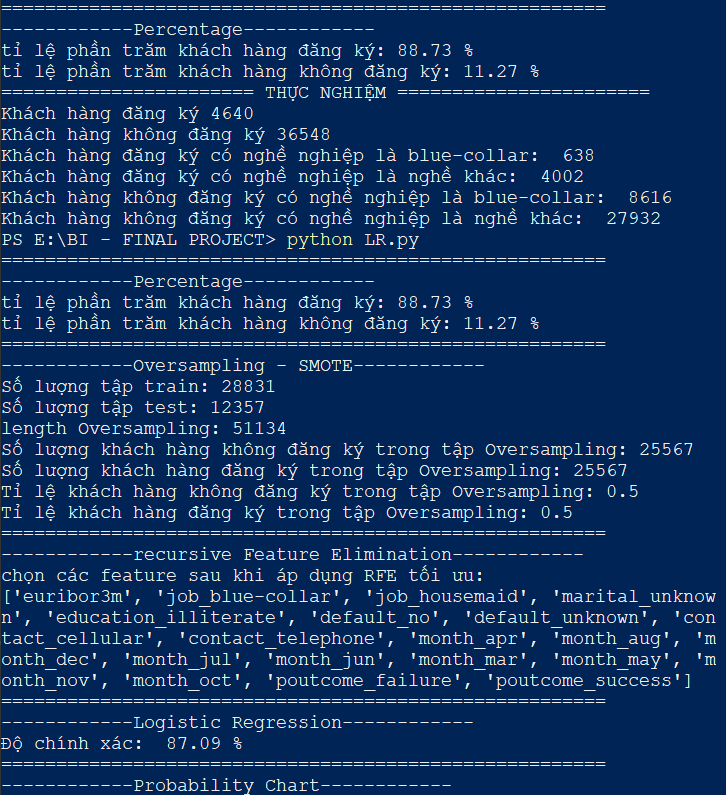
\includegraphics[scale = 1]{image/LR_2.png}
                \end{center}
            \end{figure}
        \end{center}
    
    %-------------------------------------------------------------------------------------------------------------
    \pagebreak
    %-------------------------------------------------------------------------------------------------------------
    
    \fontsize{16}{10}\selectfont
    \section{Đồ thị hóa}
        \begin{figure}[htp]
            \begin{center}
                \tab[1cm]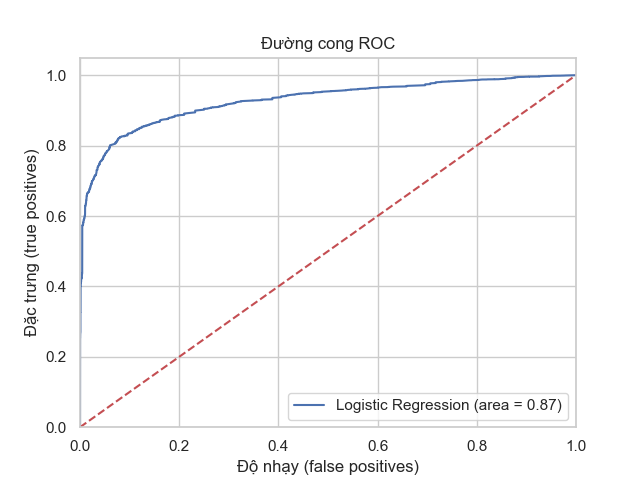
\includegraphics[scale = 0.85]{image/roc.png}
                \caption{Đồ thị đường cong góc}
            \end{center}
        \end{figure}
    
        \fontsize{13}{10}\selectfont \textbf{$\star$\textit{ Đánh giá}}
            \begin{enumerate}
                \item [- ] Đường cong ROC dùng để đánh giá các kết quả của một dự đoán.
                \item [- ] Ta thấy đường cong càng đi dọc theo biên trái và đi dọc biên phía trên của không gian ROC, kết quả kiểm tra càng chính xác.
                \item [- ] Đường cong tiến xa so với đường chéo 45 độ trong không gian ROC, độ chính xác của thuật toán trên càng chính xác.
                \item [- ] Độ chính xác của thuật toán đạt 87\%, đây là một ngưỡng khá cao.
            \end{enumerate}
            
%-------------------------------------------------------------------------------------------------------------
%---------------Chapter 4 -----------------------
\fontsize{18}{10}\selectfont
\chapter{THUẬT TOÁN MULTILAYER PERCEPTRON}
\fontsize{16}{2}\selectfont
    \section{Đôi nét về Perceptron learning algorithm (PLA), Perceptron đa tầng (Multilayer perceptron) và lan truyền ngược Backpropagation}
        \fontsize{15}{10}\selectfont\subsection{Perceptron learning algorithm (PLA)}
            \fontsize{13}{10}\selectfont\paragraph{}
                Perceptron là một thuật toán Classification cho trường hợp đơn giản nhất: chỉ có hai class (lớp) (bài toán với chỉ hai class được gọi là binary classification) và cũng chỉ hoạt động được trong một trường hợp rất cụ thể. Tuy nhiên, nó là nền tảng cho một mảng lớn quan trọng của Machine Learning là Neural Networks và sau này là Deep Learning.
                    \begin{wrapfigure}{l}[-0.65cm]{0.25\linewidth}
                        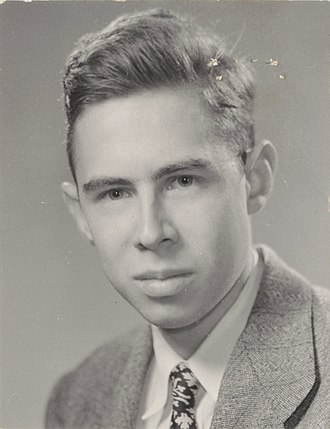
\includegraphics[scale=0.35]{image/330px-Rosenblatt_21.jpg}
                        \caption{\centering Frank Rosenblatt}
                    \end{wrapfigure}\leavevmode
                    
                    \fontsize{13}{10}\selectfont
                        Đồng thời, perceptron cũng là một thuật toán supervised learning giúp giải quyết bài toán phân lớp nhị phân, được khởi nguồn bởi Frank Rosenblatt năm 1957 trong một nghiên cứu được tài trợ bởi Văn phòng nghiên cứu hải quân Hoa Kỳ (U.S Office of Naval Research – từ một cơ quan liên quan đến quân sự).
                    \vspace{0.1cm}\paragraph{}\tab[0.5cm]\fontsize{13}{10}\selectfont
                        Perceptron được chứng minh rằng chỉ hoạt động nếu dữ liệu là linearly separable. Phát hiện này khiến cho các nghiên cứu về perceptron bị gián đoạn gần 20 năm. Thời kỳ này còn được gọi là Mùa đông AI thứ nhất (The First AI winter).\paragraph{}\leavevmode\\\leavevmode\\

            \fontsize{15}{10}\selectfont
            \subsection{Perceptron đa tầng (Multilayer perceptron)}
                \begin{wrapfigure}{l}[-0.65cm]{0.25\linewidth}
                    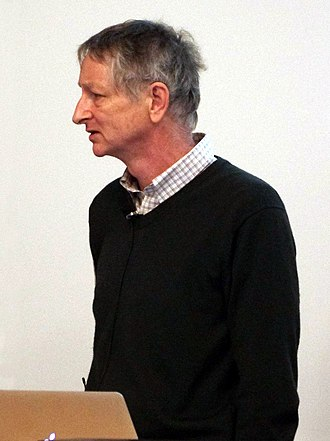
\includegraphics[scale=0.34]{image/330px-Geoffrey_Hinton_at_UBC.jpg}
                    \caption{\centering Geoffrey Hintonn}
                \end{wrapfigure}\leavevmode
                \tab[0.5cm]\fontsize{13}{10}\selectfont\paragraph{}
                    Geoffrey Hinton tốt nghiệp PhD ngành neural networks năm 1978. Năm 1986, ông cùng với hai tác giả khác xuất bản một bài báo khoa học trên Nature với tựa đề “Learning representations by back-propagating errors”. Trong bài báo này, nhóm của ông chứng minh rằng neural nets với nhiều hidden layer (được gọi là multi-layer perceptron hoặc MLP) có thể được huấn luyện một cách hiệu quả dựa trên một quy trình đơn giản được gọi là backpropagation.\paragraph{}\leavevmode\\\leavevmode\\\leavevmode\newline\leavevmode\leavevmode\\

            \fontsize{15}{10}\selectfont
            \subsection{Lan truyền ngược Backpropagation}
                \fontsize{13}{10}\selectfont
                    Backpropagation là tên gọi của quy tắc chuỗi – chain rule – trong tính đạo hàm. Việc tính được đạo hàm của hàm số phức tạp mô tả quan hệ giữa đầu vào và đầu ra của một neural network là rất quan trọng vì hầu hết các thuật toán tối ưu đều được thực hiện thông qua việc tính đạo hàm.
                        
%-------------------------------------------------------------------------------------------------------------
\pagebreak
%-------------------------------------------------------------------------------------------------------------    
    \fontsize{16}{10}\selectfont
    \section{Mô hình perceptron đa tầng (Multilayer Perceptron}
        \subsection{Các ký hiệu và khái niệm của perceptron}
            \begin{center}
                \begin{figure}[htp]
                    \begin{center}
                        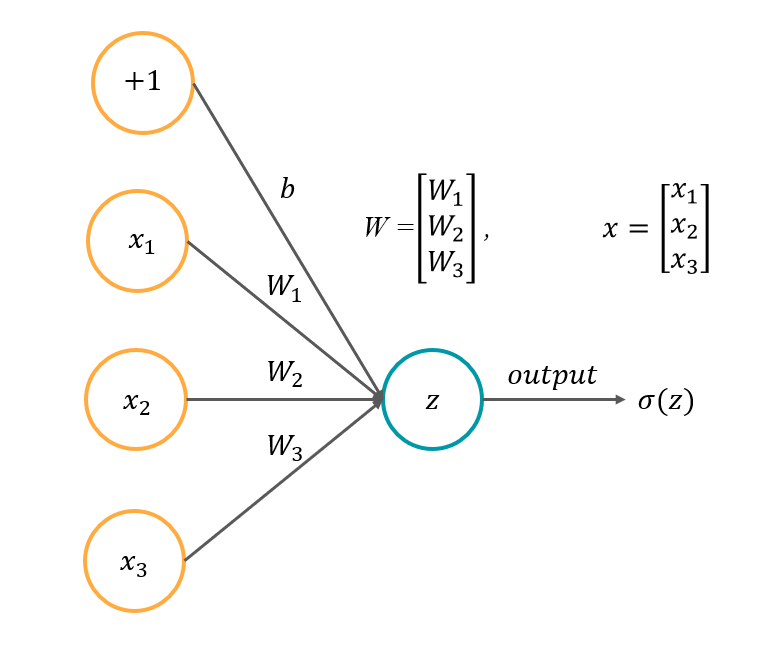
\includegraphics[scale = 0.6]{image/MLP_2.png}
                        \caption{Mô hình perceptron}
                    \end{center}
                \end{figure}
            \end{center}
            
            \begin{enumerate}
                \item [- ] $x_1, x_2, x_3$ là input của mô hình và b là giá trị bias.
                \item [- ] $W_1, W_2, W_3$ là trọng số của mô hình hay là mức độ quan trọng giá trị.
                \item [- ] z là một hàm tuyến tính có công thức như sau: $$z = W^T x + b$$ 
                \item [- ] $\sigma$(S) là hàm sigmoid (activation fuction) để chuẩn hóa output:
                \vspace{0.2cm}\newline\tab[6cm] $\sigma$(S) = $\frac{1}{1 + e^{-z}}$
            \end{enumerate}

%-------------------------------------------------------------------------------------------------------------
\pagebreak
%------------------------------------------------------------------------------------------------------------- 
        \fontsize{15}{10}\selectfont
        \subsection{Perceptron đa tầng (Multilayer Perception)}
            \begin{center}
                \begin{figure}[htp]
                    \begin{center}
                        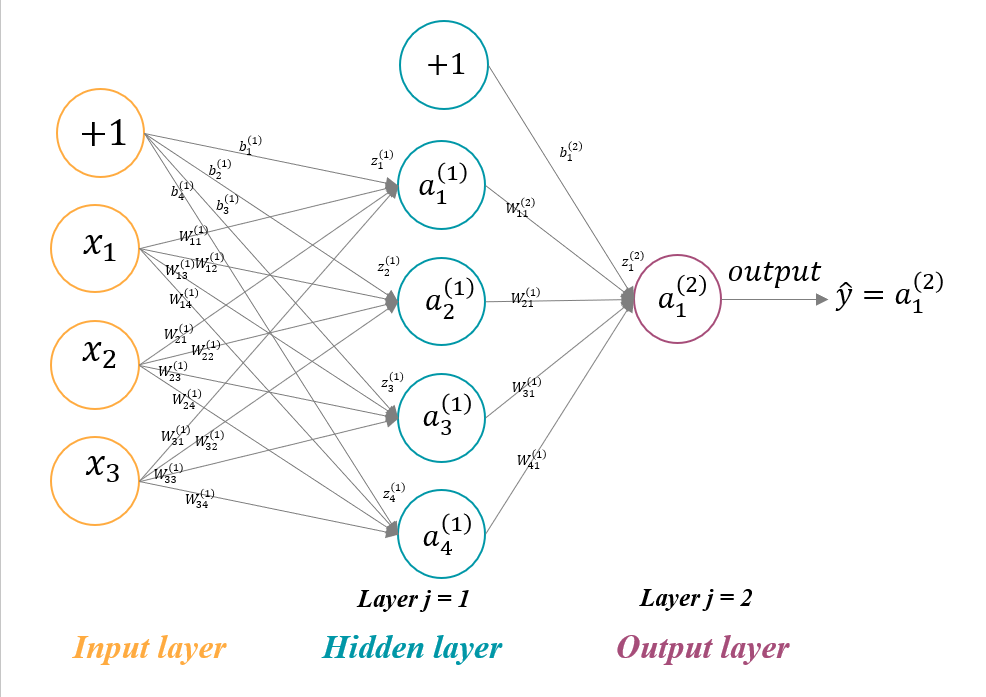
\includegraphics[scale = 0.6]{image/MLP_1.png}
                        \caption{Mô hình perceptron đa tầng (MultiLayer Perception )}
                    \end{center}
                \end{figure}
            \end{center}
            
            \begin{enumerate}
                \item [- ] Perceptron đa tầng (MLP): tập hợp của các perceptron chia làm nhiều nhóm, mỗi nhóm tương ứng với một layer. Trong hình trên có một MLP gồm 3 lớp: input layer, hidden layer, output layer.
                \item [- ] Số lượng layer trong một MLP được tính bằng số hidden layers cộng với 1. Tức là khi đếm số layers của một MLP, không tính input layers. Số lượng layer trong một MLP thường được ký hiệu là L. Trong hình trên L = 2.
                \item [- ] Mỗi vòng tròn là một node, node trong hidden layer và output layer:
                    \begin{itemize}
                        \item Được liên kết với tất cả các node ở layer trước đó với các trọng số Weight (W) riêng biệt.
                        \item Mỗi node có 1 hệ số bias (b) riêng.
                        \item Được diễn ra 2 bước: tính tổng linear và áp dụng activation function.
                    \end{itemize}
                \item [- ] $a_i^{(j)}$ là hàm kích hoạt của nút thứ i trong lớp j.
            \end{enumerate}

%-------------------------------------------------------------------------------------------------------------
\pagebreak
%------------------------------------------------------------------------------------------------------------- 
            \fontsize{13}{10}\selectfont\textbf{$\blacktriangleright$ \underline{\underline{{Biểu diễn kết quả output}}}}:
            \begin{center}
                $W_i^{(j)} = 
                \begin{bmatrix}
                    W_{1i}^{(j)} \\ W_{2i}^{(j)} \\ W_{3i}^{(j)} \\ W_{4i}^{(j)} \\ 
                \end{bmatrix}, \tab[1cm] a^{(j)} = 
                \begin{bmatrix}
                    a_{1i}^{(j)} \\ a_{2i}^{(j)} \\ a_{3i}^{(j)} \\ a_{4i}^{(j)} \\ 
                \end{bmatrix}$
            \end{center}
            
            \tab[1cm]$z_1^{(1)} = W_1^{{(1)}^T} x + b_1^{(1)}$ \tab[6cm]$z_2^{(1)} = W_2^{{(1)}^T} x + b_2^{(1)}$\\
            \tab[1.75cm]$a_1^{(1)} =\sigma (z_1^{(1)})$ \tab[7.25cm]$a_2^{(1)} =\sigma (z_2^{(1)})$\\\\
            \tab[1.5cm]$z_3^{(1)} = W_3^{{(1)}^T} x + b_3^{(1)}$ \tab[6cm]$z_4^{(1)} = W_4^{{(1)}^T} x + b_4^{(1)}$\\
            \tab[1.75cm]$a_3^{(1)} =\sigma (z_3^{(1)})$ \tab[7.25cm]$a_4^{(1)} =\sigma (z_4^{(1)})$
            
            \begin{center}
                $z_1^{(2)} = W_1^{(2)} a^{(1)} + b_1^{(2)}$\\
                $output = \hat{y} = a_1^{(2)} = \sigma (z_1^{(2)}) $
            \end{center}
            \fontsize{13}{10}\selectfont\paragraph{}\tab[0.75cm]Đây còn được gọi là phương pháp Forwardpropagation.
        
        \fontsize{15}{10}\selectfont
        \subsection{Lan truyền ngược (Backpropagation)}
            \fontsize{13}{10}\begin{enumerate}
                \item [- ] Backpropagation là phương pháp đi ngược về các layer để thay đổi giá trị của các trọng số hay giá trị bias để tối ưu lỗi của giá trị dự đoán. 
                \item [- ] Lặp đi lặp lại việc cập nhật giá trị và giảm lỗi thì cuối cùng chúng ta tạo ra một mạng có thể dự đoán tốt hơn.
                \item [- ] Để tối ưu lỗi, ta tối ưu hàm cost mà hàm cost nhận giá trị của $\hat{y}$: 
                                            $$C(\hat{y}) = -(y\log(\hat{y}) + (1 - y)\log(1 - \hat{y}))$$
                \item [- ] Hàm $\hat{y}$ nhận giá trị của z:
                                            $$\hat{y} = a(z) = \frac{1}{1+e^{-z}}$$
                \item [- ] Hàm z nhận giá trị của W,x và b:
                                            $$z = W^T x + b$$
                                            
                %-------------------------------------------------------------------------------------------------------------
                \pagebreak
                %------------------------------------------------------------------------------------------------------------- 
                \item [- ] W và b sẽ ảnh hưởng tới giá trị ouput $\hat{y}$.  Áp dụng Gradient descent, ta cập nhật giá trị W và b đến khi nào hàm cost C($\hat{y}$) đạt ngưỡng threshold thì dừng lại:
                    \vspace{0.2cm}\newline\tab[4cm]$W_{new} = W_{old} - \alpha \frac{\partial C}{\partial W_{old}}$
                        \newline\tab[10cm](Với $\alpha$ là learning rate)
                    \vspace{0.2cm}\newline\tab[4cm]$b_{new} = b_{old} - \alpha \frac{\partial C}{\partial b_{old}}$
                \item [- ] Để tính được đạo hàm từng phần của hàm cost C với W và b, phải sử dụng Chain Rule:
                                           $$\frac{\partial C}{\partial W} = \frac{\partial C}{\partial \hat{y}}  \cdot \frac{\partial \hat{y}}{\partial z} \cdot \frac{\partial z}{\partial W}$$
                                           $$\frac{\partial C}{\partial b} = \frac{\partial C}{\partial \hat{y}}  \cdot \frac{\partial \hat{y}}{\partial z} \cdot \frac{\partial z}{\partial b}$$
                \item [- ] Sau khi biến đổi công thức Chain Rule ta có:
                                           $$\frac{\partial C}{\partial z^{(L)}} = a^{(L)} - y$$
                                           $$\frac{\partial C}{\partial W^{(l)}} = a^{{l-1}^T} \cdot \frac{\partial C}{\partial z^{(l)}}$$
                                           $$\frac{\partial C}{\partial b^{(l)}} = \frac{\partial C}{\partial z^{(l)}}$$
            \end{enumerate}
    
    \fontsize{16}{10}\selectfont
    \section{Demo}
        \fontsize{15}{10}\selectfont
        \subsection{Thiết lập số liệu cần thiết}
            \begin{enumerate}
                \item [- ] Chọn learning rate = 0.00001.
                \item [- ] Số epoches = 20.
                \item [- ] Input layer, output layer va 3 hidden layer lần lượt có các số node 61, 61, 61, 61, 1.
                \item [- ] Mỗi batch chứa size = 511.
                \item [- ] Số lần learn (iterations) = 100.
                \item [- ] Phân tỉ lệ tập train với test với tỉ lệ 70:30.
            \end{enumerate}
            
        \fontsize{15}{10}\selectfont
        \subsection{Thực nghiệm}
            \begin{enumerate}
                \item [- ] Huấn luyện thuật toán trên tập train, ta được kết quả:
                    \begin{center}
                        \begin{figure}[htp]
                            \begin{center}
                                \tab[1cm]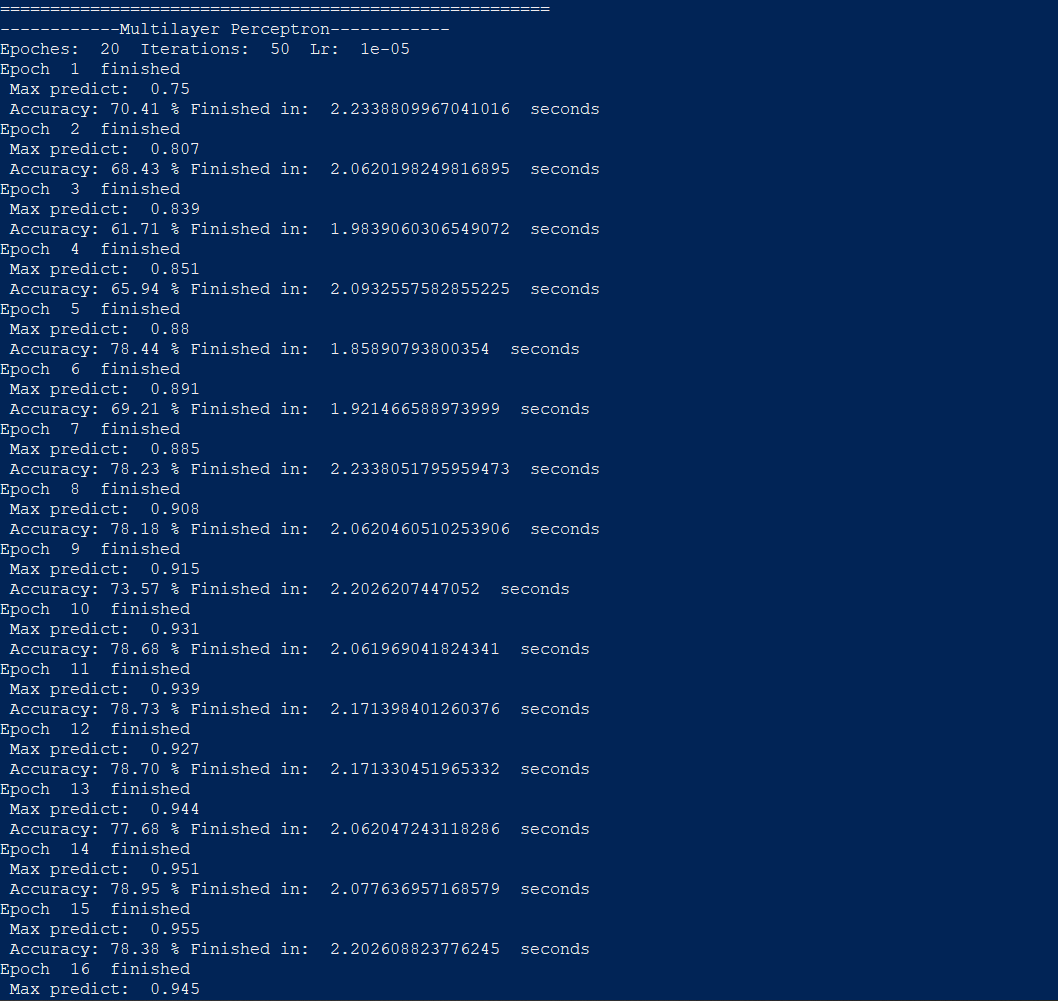
\includegraphics[scale = 0.7]{image/MLP.png}
                                \caption{Kết quả sau khi huấn luyện thuật toán trên tập train}
                            \end{center}
                        \end{figure}
                    \end{center}
                    
                %-------------------------------------------------------------------------------------------------------------
                \pagebreak
                %------------------------------------------------------------------------------------------------------------- 
                
                \item [- ] Kiểm tra 10 vị trí ngẫu nhiên trong tập test, ta được kết quả:
                    \begin{center}
                        \begin{figure}[htp]
                            \begin{center}
                                \tab[1cm]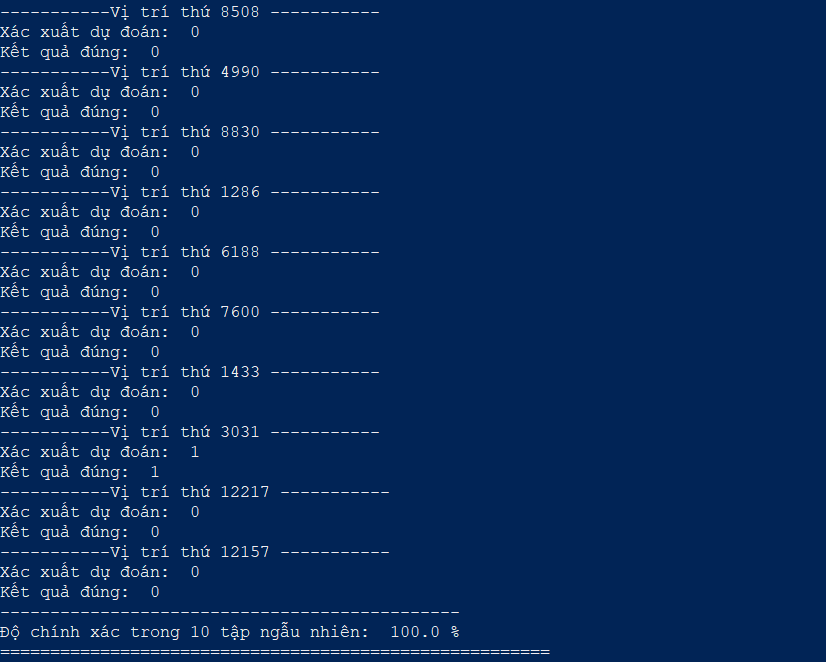
\includegraphics[scale = 0.9]{image/MLP1.png}
                                \caption{Kết quả sau khi kiểm tra ngẫu nhiên 10 vị trí trong tập test}
                            \end{center}
                        \end{figure}
                    \end{center}
            \end{enumerate}
        
        \begin{center}
            \begin{figure}[htp]
            \fontsize{15}{10}\selectfont
            \subsection{Đồ thị}
                \fontsize{14}{10}\selectfont
                \subsubsection{a) Đồ thị mất mát}
                \begin{center}
                    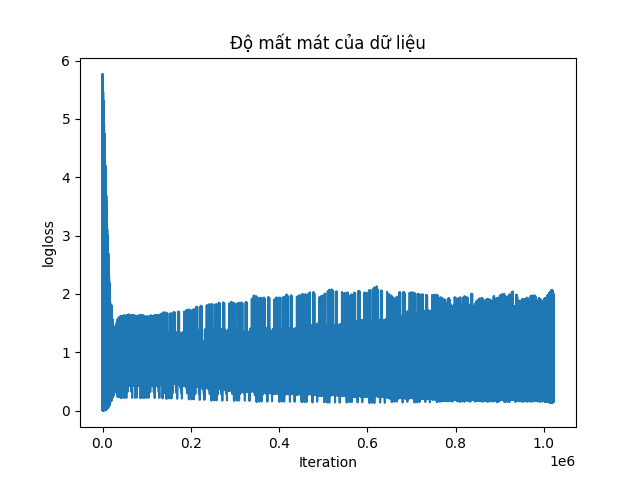
\includegraphics[scale = 0.7]{image/plot_loss_mlp.png}
                    \caption{Đồ thị thể hiện độ mất mát của dữ liệu}
                \end{center}
                \fontsize{13}{10}\selectfont \textbf{$\star$\textit{ Đánh giá}}: Sau khi áp dụng phương pháp lan truyền ngược (Backpropagation), giá trị lỗi được giảm qua từng lần learn khác nhau (iteration).
            \end{figure}
        \end{center}
        
        \begin{center}
            \begin{figure}[htp]
                \fontsize{14}{10}\selectfont
                \subsubsection{b) Đồ thị sự phân bố xác suất dự đoán}
                \begin{center}
                    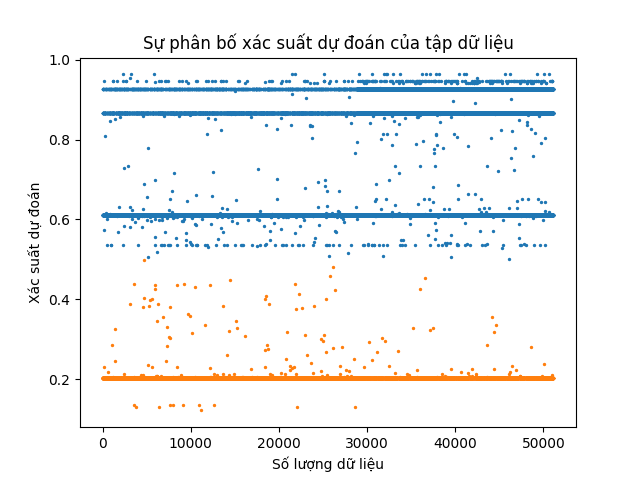
\includegraphics[scale = 0.7]{image/plot_predict_mlp.png}
                    \caption{Đồ thị thể hiện sự phân bố xác suất dự đoán của tập dữ liệu}
                \end{center}
            \end{figure}
        \end{center}
        
%-------------------------------------------------------------------------------------------------------------
%---------------Chapter 5 -----------------------        
\fontsize{18}{10}\selectfont
\chapter{THUẬT TOÁN K-NEAREST NEIGHBORS (KNN)}
    \fontsize{16}{10}\selectfont
    \section{K-Nearest Neighbors (KNN)}
        \fontsize{13}{10}\selectfont\paragraph{}
            KNN (K-Nearest Neighbors) là một trong những thuật toán học có giám sát đơn giản nhất được sử dụng nhiều trong khai phá dữ liệu và học máy. Ý tưởng của thuật toán này là nó không học một điều gì từ tập dữ liệu học (nên KNN được xếp vào loại lazy learning), mọi tính toán được thực hiện khi nó cần dự đoán nhãn của dữ liệu mới.
            \vspace{0.2cm}\newline\tab[0.4cm] Đối với thuật toán KNN thì lớp (nhãn) của một đối tượng dữ liệu mới có thể dự đoán từ các lớp (nhãn) của k hàng xóm gần nó nhất.
    
        \fontsize{15}{10}\selectfont
        \subsection{Việc ứng dụng thuật toán KNN}
            \fontsize{13}{2}\selectfont\paragraph{}
                \textit{Trong y tế}: xác định bệnh lý của người bệnh mới dựa trên dữ liệu lịch sử của các bệnh nhân có cùng bệnh lý, có cùng các đặc điểm đã được chữa khỏi trước đây, hay xác định loại thuốc phù hợp với người bệnh,...
                
            \fontsize{13}{2}\selectfont\paragraph{}
                \textit{Trong ngân hàng}: xác định khả năng khách hàng chậm trả các khoản vay hoặc rủi ro tín dụng do nợ xấu dựa trên phân tích Credit score, xác định xem liệu các giao dịch mang hành vi phạm tội, lừa đảo hay không, hay như đề tài xác định khách hàng có đăng ký một khoản tiền gửi có kỳ hạn hay không thông qua các dữ liệu thu thập từ chiến dịch tiếp thị thị trường.
                
            \fontsize{13}{2}\selectfont\paragraph{}
                \textit{Trong giáo dục}: phân loại các học sinh theo hoàn cảnh, học lực để xem xét cần hổ trợ gì cho những học sinh trên.
                     
            %-------------------------------------------------------------------------------------------------------------
            \pagebreak
            %-------------------------------------------------------------------------------------------------------------
    
            \fontsize{13}{2}\selectfont\paragraph{}
                \textit{Trong thương mại điện tử}: phân loại khách hàng theo sở thích cụ thể để xây dựng hệ thống khuyến nghị, dựa trên dữ liệu từ website, app,...
            \fontsize{13}{2}\selectfont\paragraph{}
                \textit{Trong kinh tế}: giúp dự báo các sự kiện kinh tế trong tương lai, dự báo tình hình thời tiết trong nông nghiệp, xác định xu hướng thị trường chứng khoán,…
            
        \fontsize{15}{10}\selectfont
        \subsection{Ưu - nhược điểm của thuật toán}
            \begin{enumerate}
                \item [- ] Ưu điểm:
                    \begin{itemize}
                        \item Thuật toán đơn giản, dễ dàng triển khai.
                        \item Độ phức tạp tính toán nhỏ.
                        \item Việc dự đoán kết quả của dữ liệu mới rất đơn giản.
                        \item Không cần giả sử phân phối của các class.
                        \item Xử lý tốt với tập dữ liệu bị nhiễu.
                    \end{itemize}
                \item [- ] Nhược điểm:
                    \begin{itemize}
                        \item Với k điểm nhỏ, dễ gặp nhiễu dẫn tới kết quả đưa ra không chính xác.
                        \item Cần nhiều thời gian để thực hiện thuật toán do phải tính toán khoảng cách với tất cả các đối tượng trong tập dữ liệu.
                        \item Cần chuyển đổi dữ liệu thành các yếu tố định tính.
                        \item Việc lưu toàn bộ dữ liệu trong bộ nhớ ảnh hưởng tới hiệu năng của KNN.
                        \item Độ phức tạp càng tăng khi k càng lớn.
                    \end{itemize}
            \end{enumerate}
    
    \fontsize{16}{10}\selectfont
    \section{Mô hình thuật toán K-Nearest Neighbors (KNN)}
        \begin{enumerate}
            \item [- ] Thuật toán KNN cho rằng những dữ liệu tương tự nhau sẽ tồn tại gần nhau trong một không gian, từ đó sẽ tìm k điểm gần với dữ liệu cần kiểm tra nhất. Việc tìm khoảng cách giữa 2 điểm củng có nhiều công thức có thể sử dụng, tùy trường hợp mà lựa chọn phù hợp. Có 3 cách cơ bản để tính khoảng cách giữa 2 điểm dữ liệu x, y có k thuộc tính:
                \begin{center}
                    \begin{figure}[htp]
                        \begin{center}
                            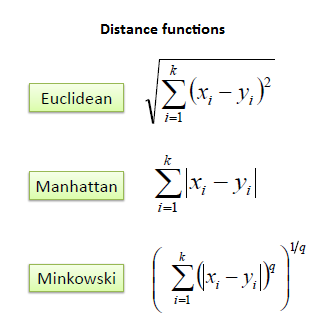
\includegraphics[scale = 1.2]{image/Distance.png}
                            \caption{Công thức cơ bản để tính khoảng cách giữa hai điểm dữ liệu x và y}
                        \end{center}
                    \end{figure}
                \end{center}    
                
            %-------------------------------------------------------------------------------------------------------------
            \pagebreak
            %------------------------------------------------------------------------------------------------------------- 
            
            \item [- ] Các bước xây dựng một mô hình KNN:
                \item Giả sử D là tập các điểm dữ liệu đã được phân loại và C là dữ liệu chưa được phân loại.
                \item Đo khoảng cách (Euclidian, Manhattan, Minkowski) từ dữ liệu C đến tất cả điểm dữ liệu khác đã được phân loại trong D.
                \item Chọn K là số điểm có khoảng cách gần nhất với C.
                \item Kiểm tra danh sách các lớp có khoảng cách ngắn nhất và đếm số lượng mỗi lớp xuất hiện.
                \item Lấy đúng lớp xuất hiện nhiều lần nhất trong tập K điểm gần nhất.
                \item Lớp của dữ liệu C là lớp chọn từ bước 5.
        \end{enumerate}
        
    %-------------------------------------------------------------------------------------------------------------
    \pagebreak
    %------------------------------------------------------------------------------------------------------------- 
    
    \fontsize{16}{10}\selectfont
    \section{Thực nghiệm trên đề tài}
        \fontsize{13}{10}\selectfont
        \begin{enumerate}
            \item [- ] Xét 15 tập dữ liệu trên đề tài (chọn 4 biến độc lập)
                \begin{center}
                    \begin{figure}[htp]
                        \begin{center}
                            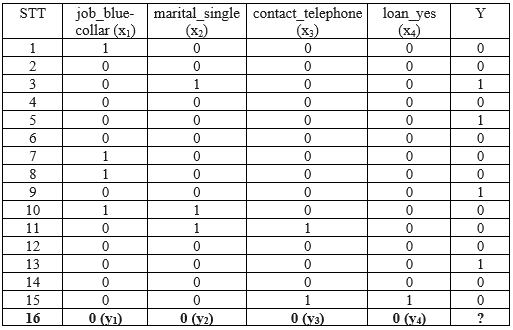
\includegraphics[scale = 1]{image/input_thucnghiem.PNG}
                        \end{center}
                    \end{figure}
                \end{center}
                
            \item [- ] Áp dụng hàm Euclidean tính distance (khoảng cách):
                $$D = \sqrt{(x_1 - y_1)^2 + (x_2 - y_2)^2 + (x_3 - y_3)^2 + (x_4 - y_4)^2}$$
                \begin{center}
                    \begin{figure}[htp]
                        \begin{center}
                            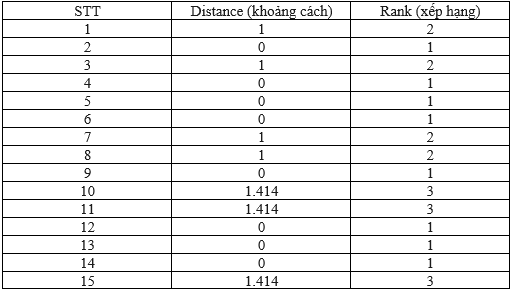
\includegraphics[scale = 1]{image/result_after_using_Euclidean.PNG}
                        \end{center}
                    \end{figure}
                \end{center}
                
            %-------------------------------------------------------------------------------------------------------------
            \pagebreak
            %------------------------------------------------------------------------------------------------------------- 
        
            \item [- ] Chọn k = 5, ta được:
                \begin{center}
                    \begin{figure}[htp]
                        \begin{center}
                            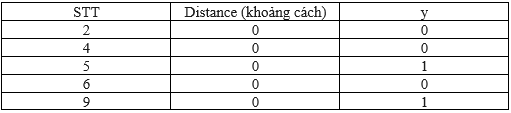
\includegraphics[scale = 1]{image/result_after_choosingK.PNG}
                        \end{center}
                    \end{figure}
                \end{center}
            \fontsize{13}{10}\selectfont\textbf{$\Longrightarrow$ \underline{\underline{{Kết luận}}}}: trong 5 tập dữ liệu được chọn, label = 0 chiếm đa số $\Rightarrow$ vậy dữ liệu số 16 được phân loại vào lớp 0.
        \end{enumerate}
        
    \fontsize{16}{10}\selectfont
    \section{Demo}
        \fontsize{13}{10}\selectfont
        \begin{enumerate}
            \item [- ] Chia tập dữ liệu thành 2 tập train, test với tỉ lệ 70:30.
            
            \item [- ] Thực hiện thuật toán áp dụng cho tập dữ liệu, ta được:
                \begin{center}
                    \begin{figure}[htp]
                        \begin{center}
                            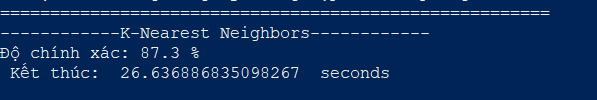
\includegraphics[scale = 1.2]{image/KNN.png}
                            \caption{Kết quả nhận được sau khi áp dụng thuật toán cho tập dữ liệu}
                        \end{center}
                    \end{figure}
                \end{center}
                
            \item [- ] Đánh giá:
                \begin{itemize}
                    \item Do việc phải tính khoảng cách của từng điểm trong tập dữ liệu, việc huấn luyện có thể diễn ra trong thời gian rất dài. Cụ thể tốn 26.64 giây để có thể tính toán ra được độ chính xác của thuật toán.
                    \item Việc chọn K rất quan trọng, nếu chọn K quá nhỏ dữ liệu ta dự đoán sẽ bị nhiều nên việc chọn K phải dựa vào tập dữ liệu và số lượng dữ liệu.
                \end{itemize}
                    
            %-------------------------------------------------------------------------------------------------------------
            \pagebreak
            %------------------------------------------------------------------------------------------------------------- 
        
            \item [- ] Dự đoán trong 10 tập dữ liệu ngẫu nhiên trong tập test:
                \begin{center}
                    \begin{figure}[htp]
                        \begin{center}
                            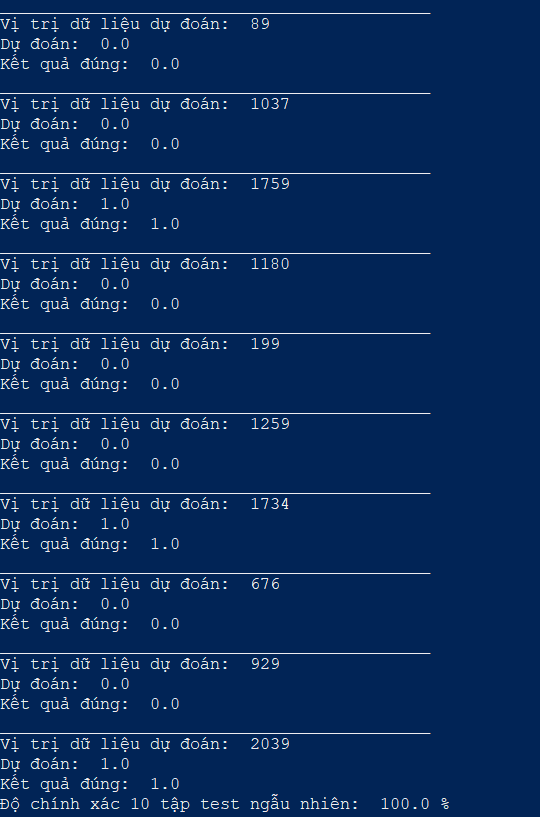
\includegraphics[scale = 0.9]{image/KNN_2.png}
                            \caption{Kết quả dự đoán 10 tập dữ liệu ngẫu nhiên trong test}
                        \end{center}
                    \end{figure}
                \end{center}
        \end{enumerate}
        
%-------------------------------------------------------------------------------------------------------------
%---------------Chapter 6 -----------------------        
\fontsize{18}{10}\selectfont
\chapter{TÀI LIỆU THAM KHẢO}
    \fontsize{16}{10}\selectfont\textbf{Tiếng Việt}\vspace{0.4cm}
        \begin{enumerate}
            \item https://phantichspss.com/chi-odds-ratio-va-confidence-interval-ci-dinh-nghia-y-nghia-va-cach-tinh-toan.html
            \item https://bigdatauni.com/vi/tin-tuc/tong-quan-ve-logistic-regression-hoi-quy-logistic-phan-1.html
            \item https://machinelearningcoban.com/2017/02/24/mlp/\#-backpropagation-cho-stochastic-gradient-descent
            \item https://machinelearningcoban.com/2017/01/21/perceptron/\#bai-toan\\-perceptron
            \item https://dlapplications.github.io/2018-06-15-MLP/
            \item https://viblo.asia/p/knn-k-nearest-neighbors-1-djeZ14ejKWz
            \item https://machinelearningcoban.com/2017/01/08/knn/
        \end{enumerate}
        
    \vspace{0.4cm}\fontsize{16}{10}\selectfont\textbf{Tiếng Anh}\vspace{0.4cm}
        \begin{enumerate}
            \item https://en.wikipedia.org/wiki/Multilayer\_perceptron
            \item https://towardsdatascience.com/deep-neural-multilayer-perceptron-mlp-with-scikit-learn-2698e77155e
            \item https://scikit-learn.org/stable/auto\_examples/neighbors/plot\_regression.\\html\#sphx-glr-auto-examples-neighbors-plot-regression-py
            \item https://www.simplilearn.com/deep-learning-algorithms-article
        \end{enumerate}
\end{document}